\section{Limitations of Current Self-Verification and Aggregation Approaches}
\label{sec:why_improve}

\begin{figure}[H]
    \centering
    \begin{minipage}[t]{0.32\textwidth}
        \centering
        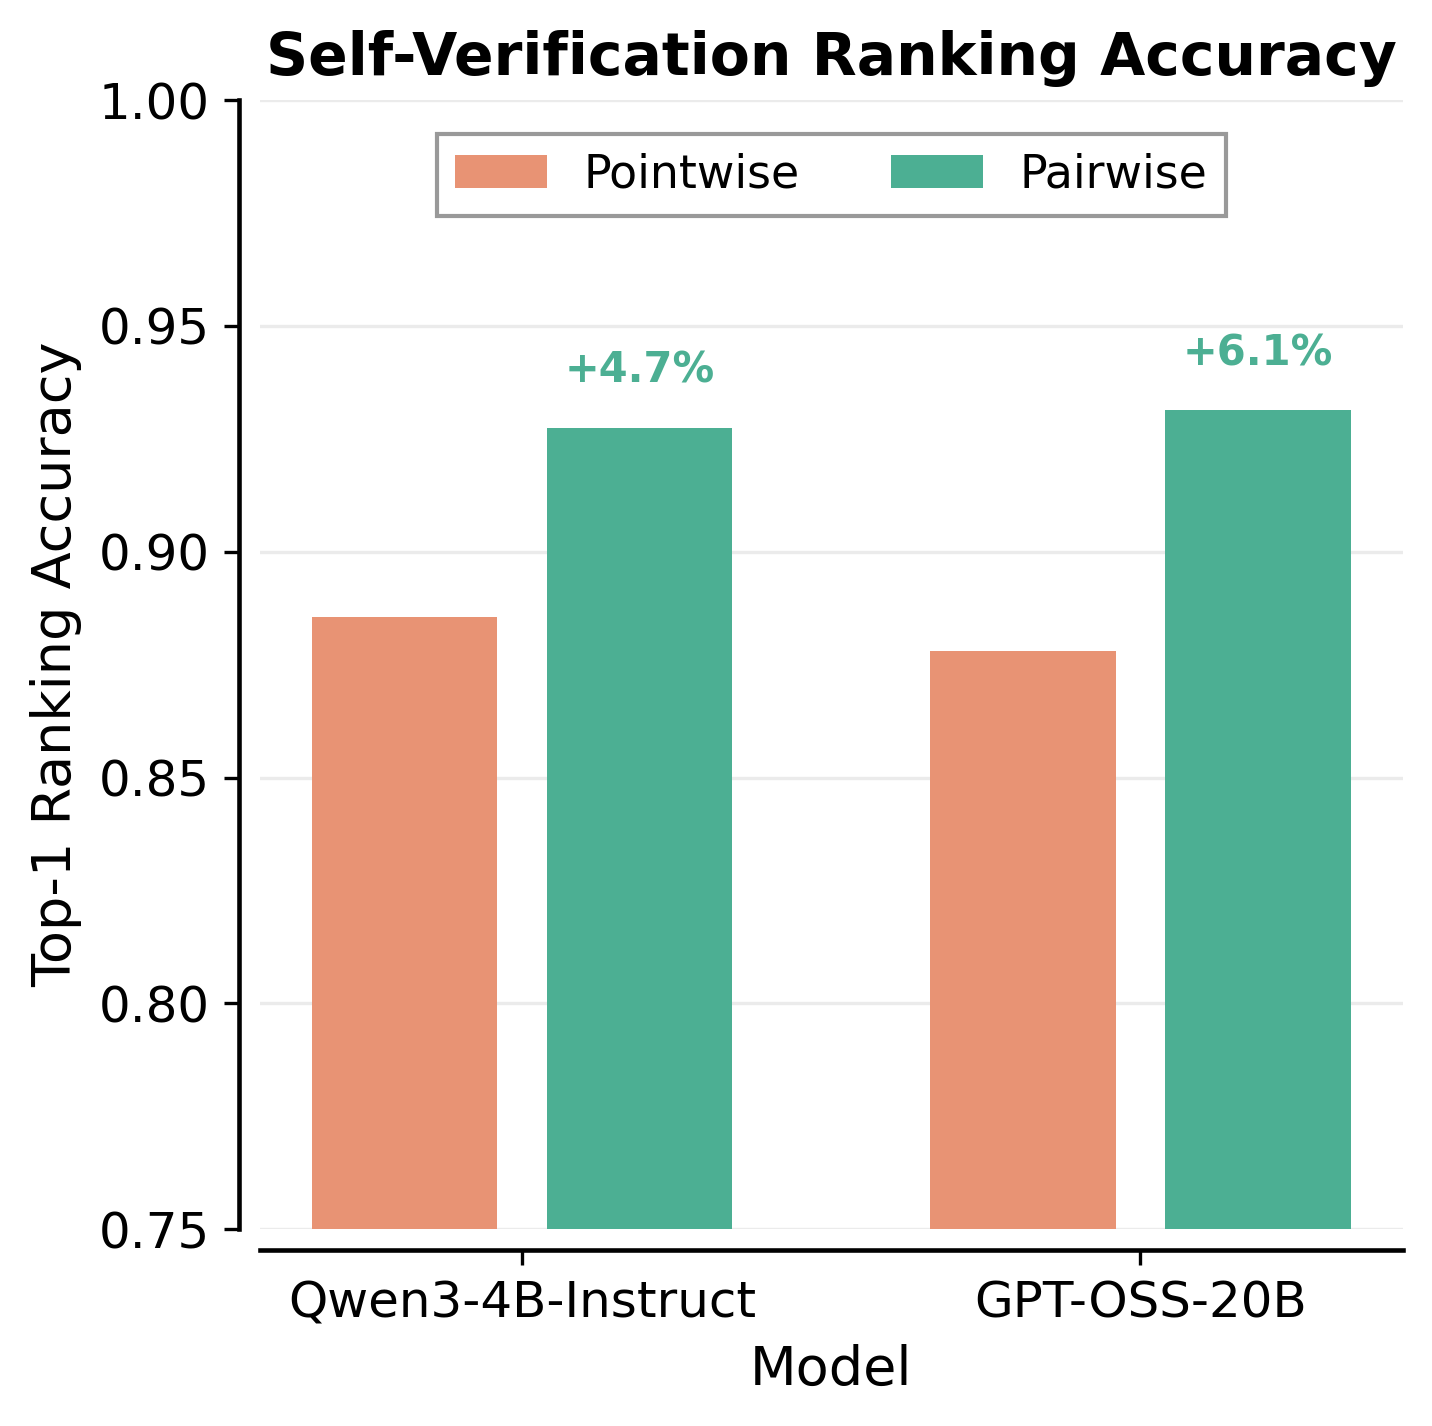
\includegraphics[width=\linewidth]{images_verif/ranking_accuracy_pointwise_vs_pairwise.png}
    \end{minipage}
    \hfill
    \begin{minipage}[t]{0.32\textwidth}
        \centering
        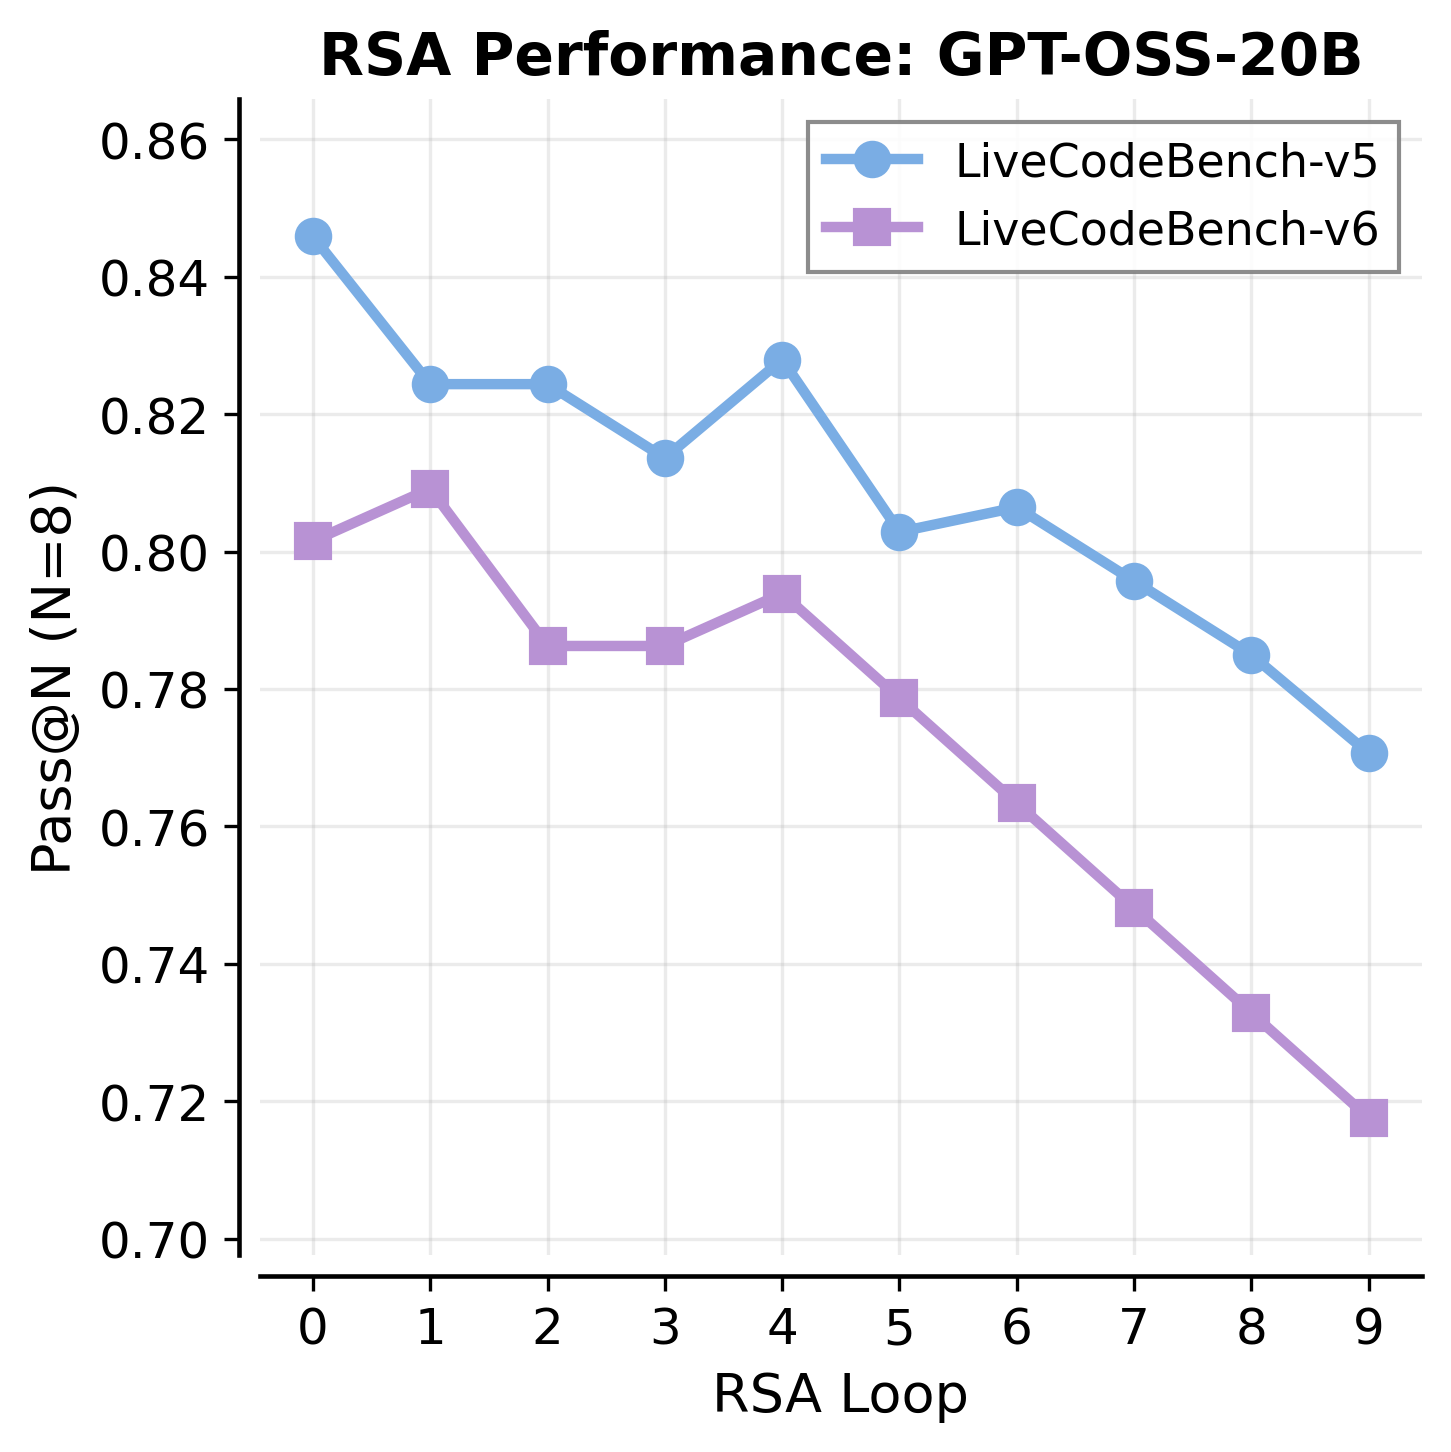
\includegraphics[width=\linewidth]{images_verif/rsa_gpt_oss_20b_lcb_comparison.png}
    \end{minipage}
    \hfill
    \begin{minipage}[t]{0.32\textwidth}
        \centering
        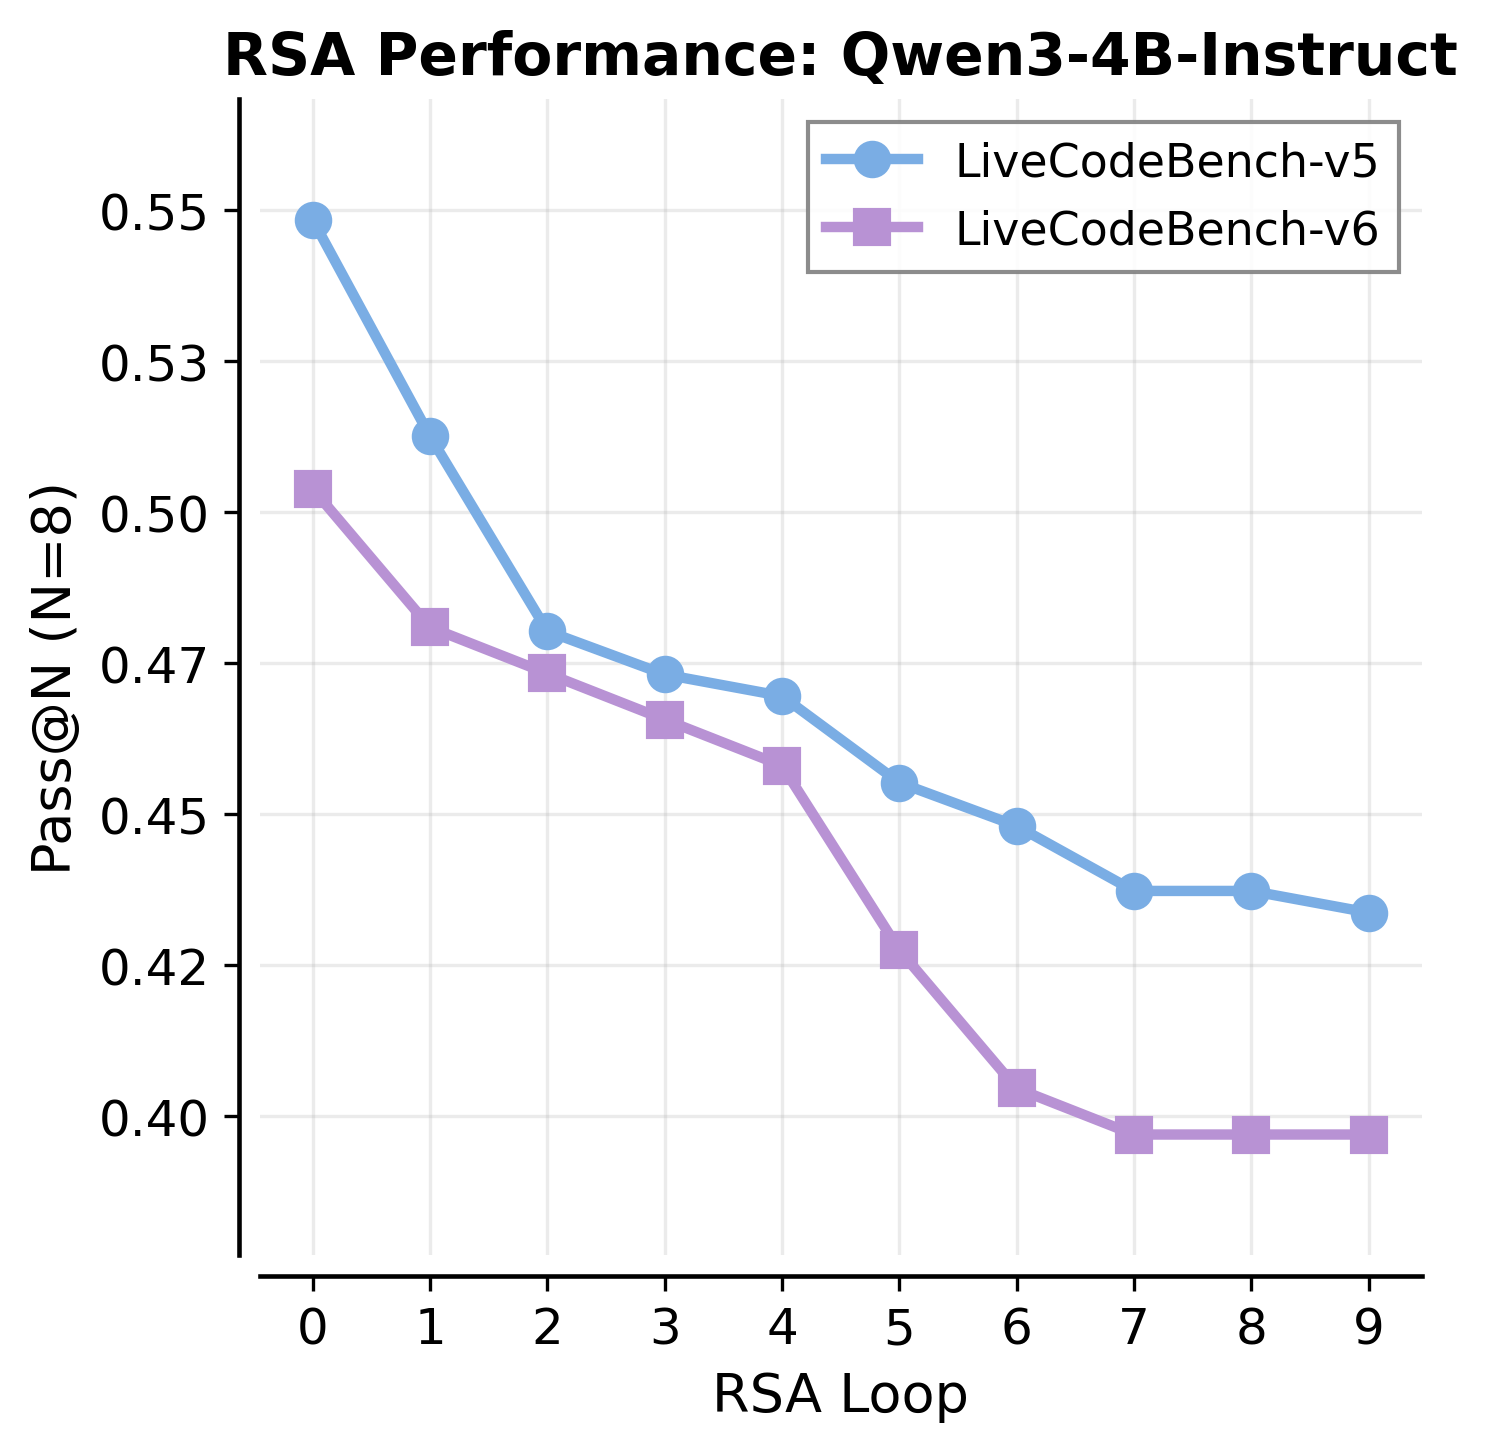
\includegraphics[width=\linewidth]{images_verif/rsa_Qwen3_4B_Instruct_2507_lcb_comparison.png}
    \end{minipage}
    \caption{
        \textbf{(Left)} Pairwise self-verification (using \pairinfer{}, \S\ref{sec:swiss_pairwise_verification}) outperforms pointwise self-verification in self-verification measured on problems which have both correct and incorrect solutions in their parallel generations (Results with GPT-OSS-20B on LiveCodeBench-V6 prompts). \textbf{(Middle and Right)} Recursive self-aggregation on LiveCodeBench benchmarks shows declining Pass@N (diversity collapse) for both GPT-OSS-20B and Qwen3-4B-Instruct. See \S\ref{sec:why_improve} for more details.
    }
    \label{fig:rsa_lcb_pass_at_n}
\end{figure}

From a test-time scaling perspective without external verifiers, parallel reasoning offers two prevalent mechanisms to generate the final solution: \textbf{a) self-selection} (verifying and choosing the best candidate) and \textbf{b) self-aggregation} (combining solutions to generate a better one). We analyze the limitations of current approaches in both categories to motivate our pairwise framework \footnote{Majority voting is less general and only applicable to scenarios with objective ground-truth answers, such as math.}.


\textbf{Pointwise self-verification suffers from calibration collapse.}
Standard pointwise verification assigns scalar scores to solutions in isolation. This approach is fundamentally limited by the lack of a comparative reference set. Statistically, latent utilities in choice models (e.g., Bradley--Terry) are identifiable only up to monotonic transformations, meaning absolute scores lack a globally comparable scale \citep{bradley1952rank}. Consequently, pointwise scores exhibit high variance and poor cross-context calibration, often over-scoring plausible but incorrect solutions. \citet{christiano2017rlhf} noted that for learning from human preferences, relative scores are much easier to provide for humans compared to absolute scores. \textit{Pairwise} judgments simplify the task to a well-posed relative comparison. As shown in Figure \ref{fig:rsa_lcb_pass_at_n} (left), this shift to relative ranking yields significantly higher top-1 self-ranking accuracy.

\textbf{Self-aggregation leads to reduction in pass@N and diversity collapse.}
Self-aggregation-based methods prompt the same LLM to consolidate parallelly generated solutions into one solution. While self-aggregation methods \citep{venkatraman2025recursiveselfaggregationunlocksdeep, khairi2025makingtakingbestn, li2025llms, madaan2025rethinkingthinkingtokensllms} can help consolidate parallel reasoning chains and improve Pass@1, they may lead to \textit{diversity collapse}. As shown in Figure \ref{fig:rsa_lcb_pass_at_n} (Middle and Right), the Pass@N score, representing the probability that \textit{at least one} correct solution exists in a set of generated N solutions, monotonically decreases as aggregation steps increase for RSA. This indicates that RSA frequently discards or degrades correct outlier solutions during refinement. Specifically, since the refined Pass@1 rarely exceeds the \textit{initial} Pass@N of the raw samples, the value of self-aggregation is unclear compared with a strong self-verifier that can select the best answer and reach near Pass@N performance. Instead of relying on implicit self-verification capabilities of aggregation based method, explicit and accurate self-verification can provide orthogonal improvements to aggregator-based approaches since each aggregation step (that may induce diversity collapse) can benefit from self-verification (that maintains pass@N), which can help select promising candidate solutions to aggregate.


\begin{tcolorbox}[title=Takeaway: Key Limitations of Existing Self-Verification and Aggregation Approaches, colback=green!5]
Pointwise self-verification lacks calibration due to the absence of comparative references, while self-aggregation methods suffer from diversity collapse that discards correct solutions during aggregation. Pairwise self-verification offers a principled orthogonal method that is both better calibrated and diversity-preserving.
\end{tcolorbox}

\begin{figure}[t]
    \centering
    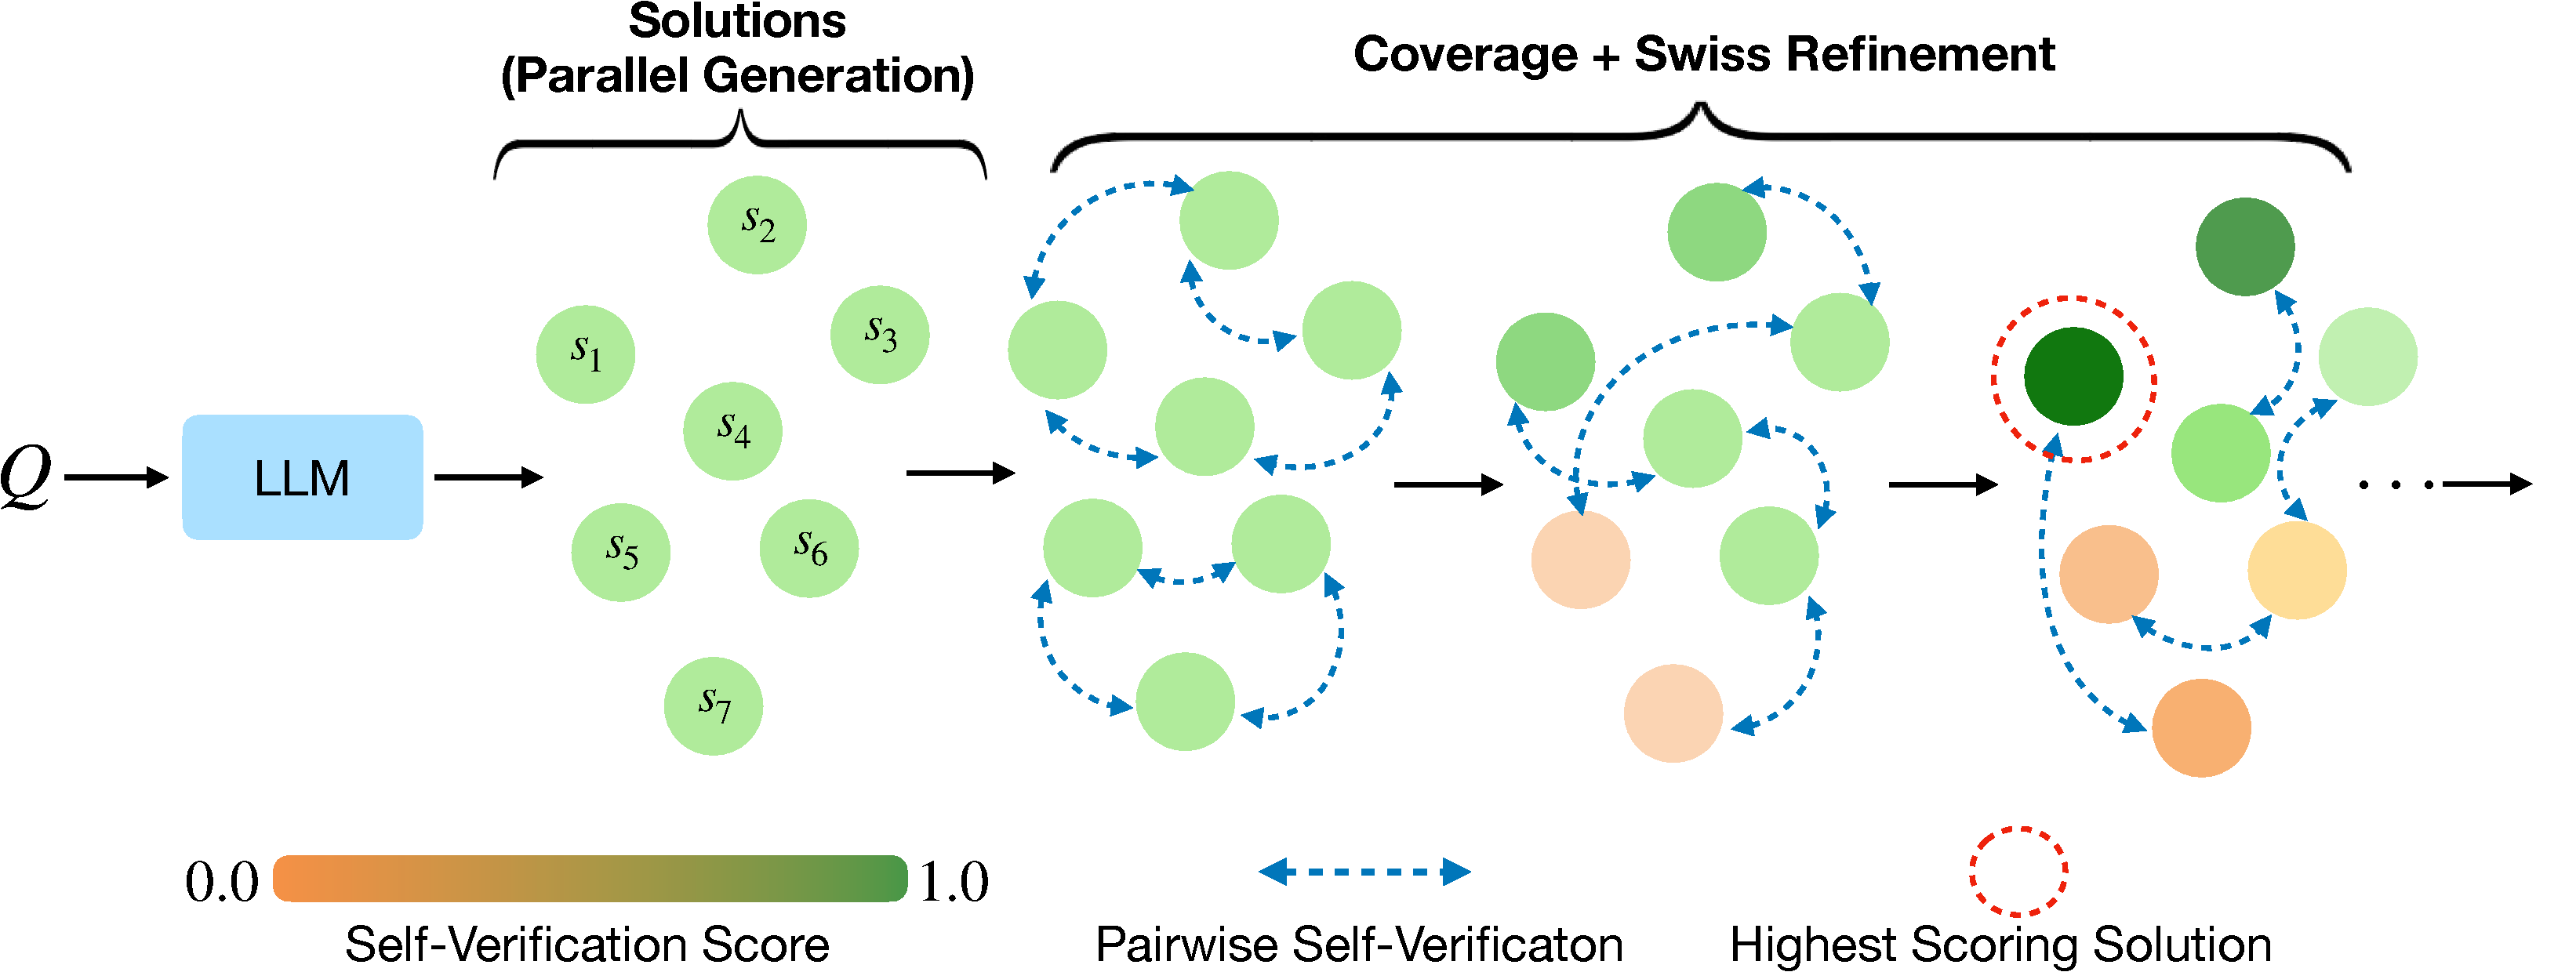
\includegraphics[width=0.88\textwidth]{figures/fig_1_plot_swiss-cropped.pdf}
    \caption{Swiss Refinement Overview. Increasing pairwise verifications enables LLMs to better self-verify for selecting the best response among N self-generated solutions. See Section~\ref{sec:swiss_pairwise_verification}}
    \label{fig:swiss_refinement_overview}
\end{figure}

\section{Improving the Self-Verification Capability of LLMs using \pairinfer{}}
\label{sec:swiss_pairwise_verification}

Pointwise verification is limited in its ability to capture relative nuances and lacks calibration.
These limitations, coupled with a desire to maintain solution diversity, motivate us to propose \textit{\pairinfer{}}, a pairwise self-verification framework designed for parallel reasoning.
While we can use pairwise self-verification to score responses by the model, naively pairing solutions may require quadratic number of $C(N,2)$ self-verification attempts. Our approach, detailed in~\cref{alg:ugpr}, consists of a weighted aggregation mechanism and a two-phase budgeting strategy designed to maximize information gain with each new pair which allows us to efficiently scale test-time self-verification compute while achieving significant improvement in reasoning performance. A high-level overview of our approach is presented in Fig.~\ref{fig:swiss_refinement_overview}


\begin{figure}[H]
    \centering
    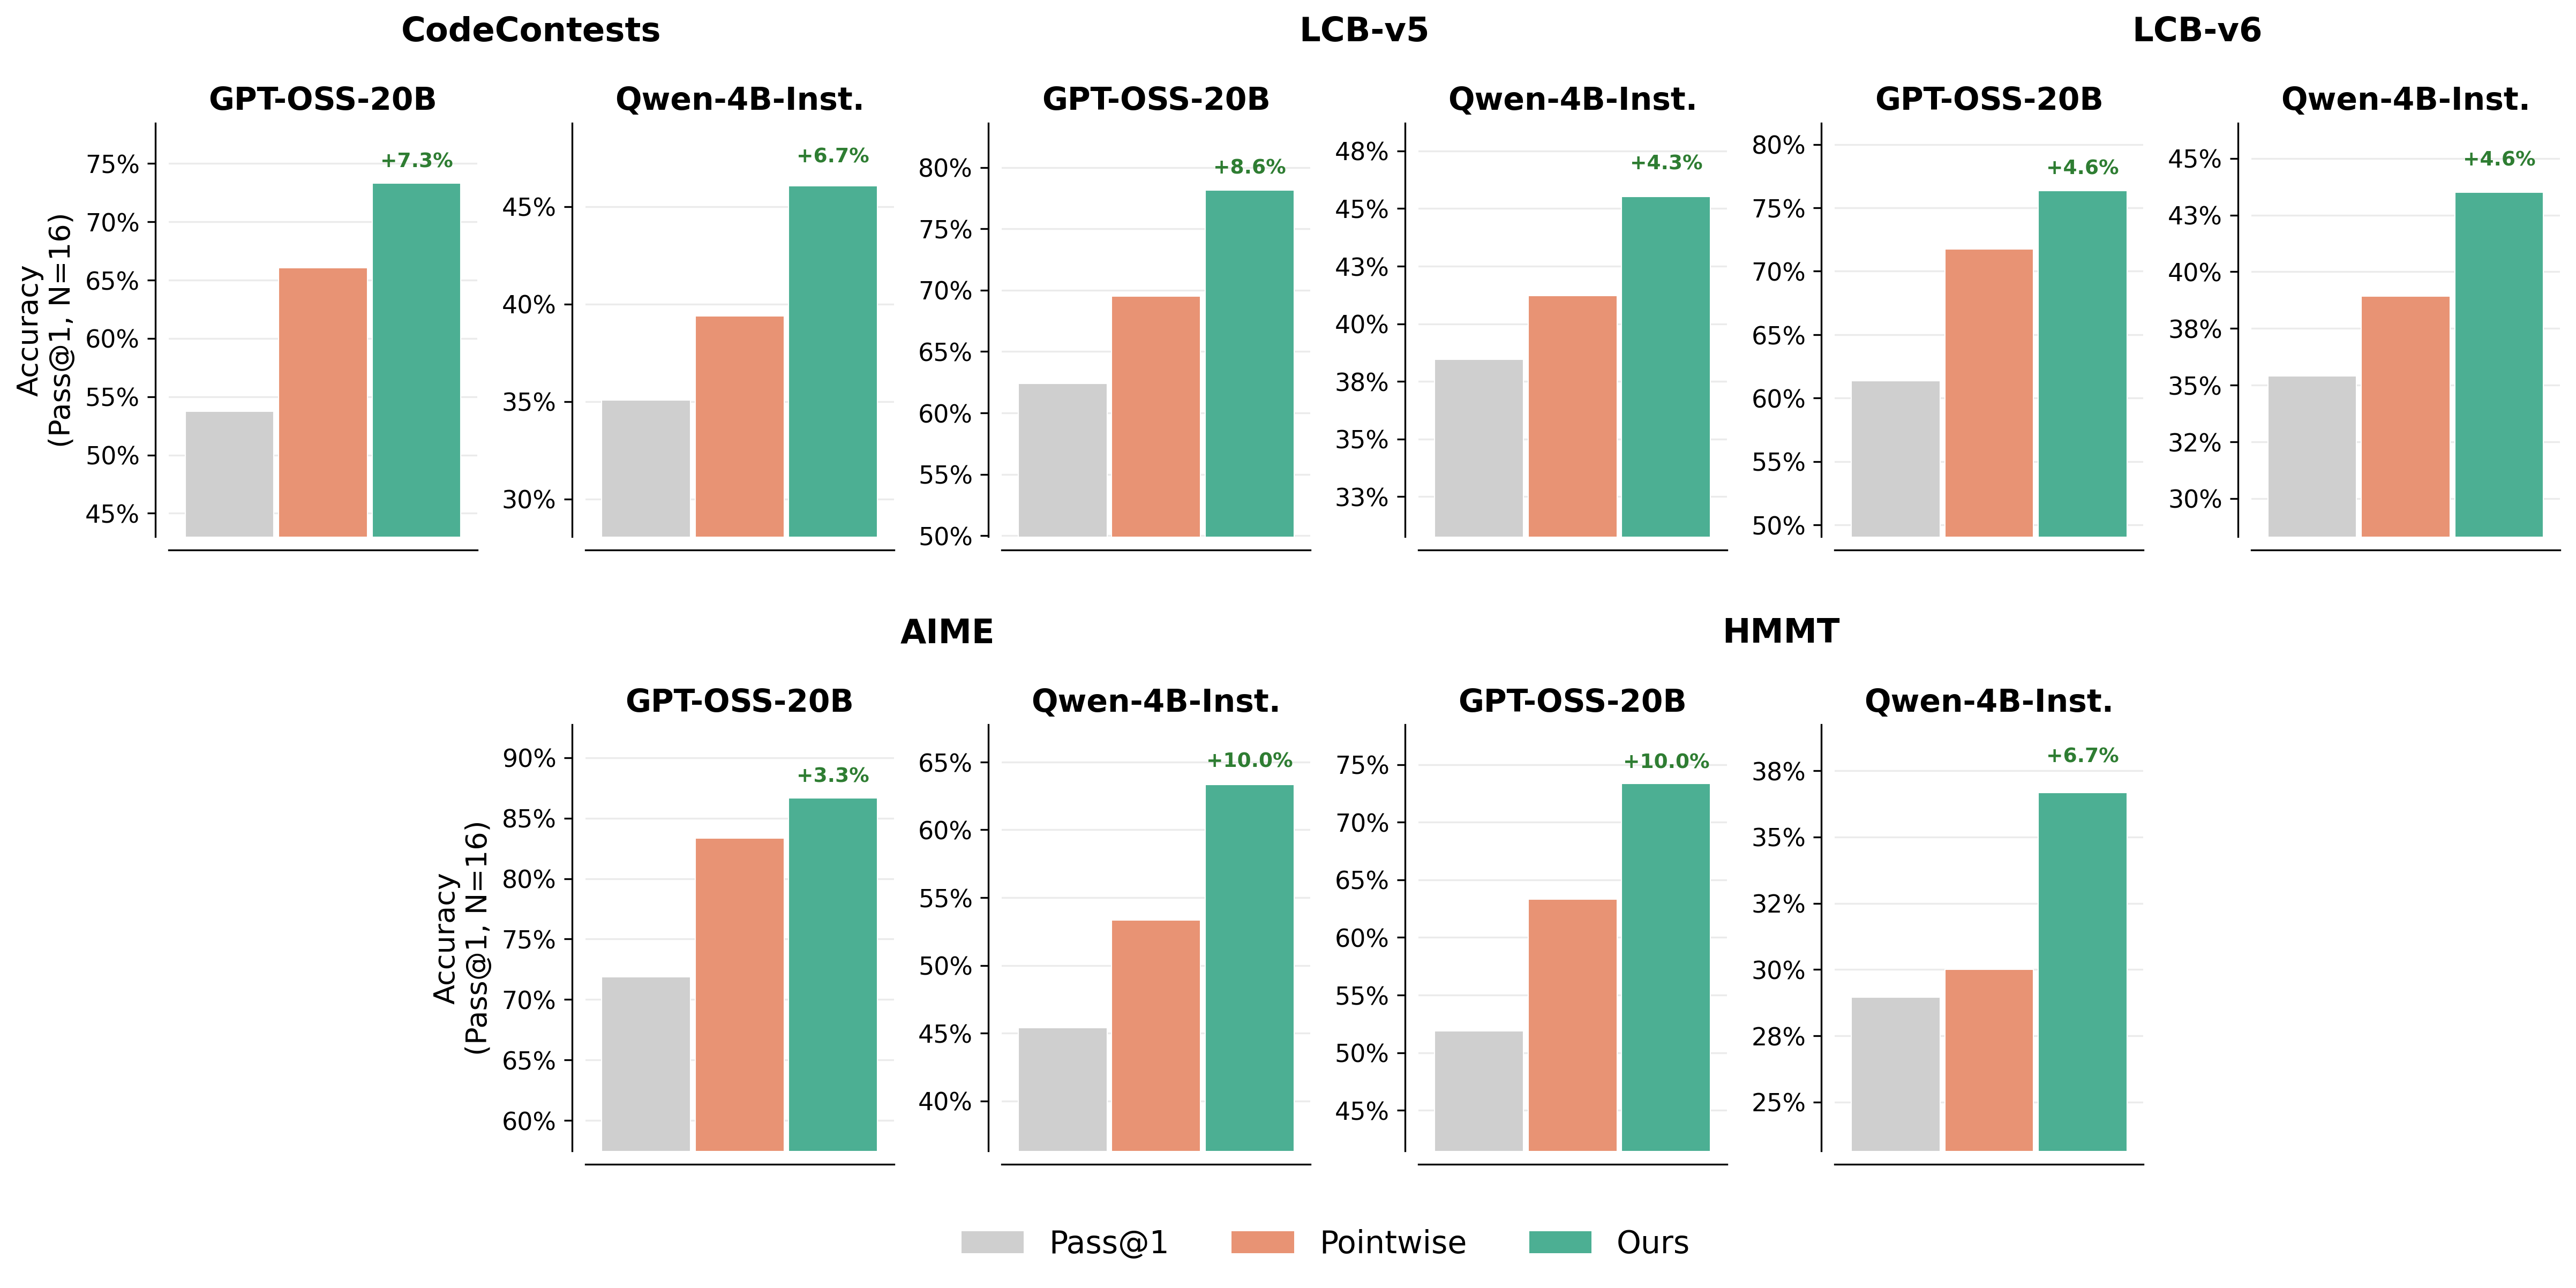
\includegraphics[width=\textwidth]{images_verif/figure1_inference_results_2row.png}
    \caption{
        Performance after self-verification using \pairinfer{} compared with pointwise self-verification across benchmarks and models at N=16 base generations. Results presented for GPT-OSS-20B and Qwen3-4B-Instruct-2507. Results for GPT-OSS-120B and Qwen3-4B-Thinking-2507 are in Fig.~\ref{fig:appendix-all-verif-bars} and show similar trends.
    }
    \label{fig:inference-results}
\end{figure}

\begin{figure}[H]
    \centering
    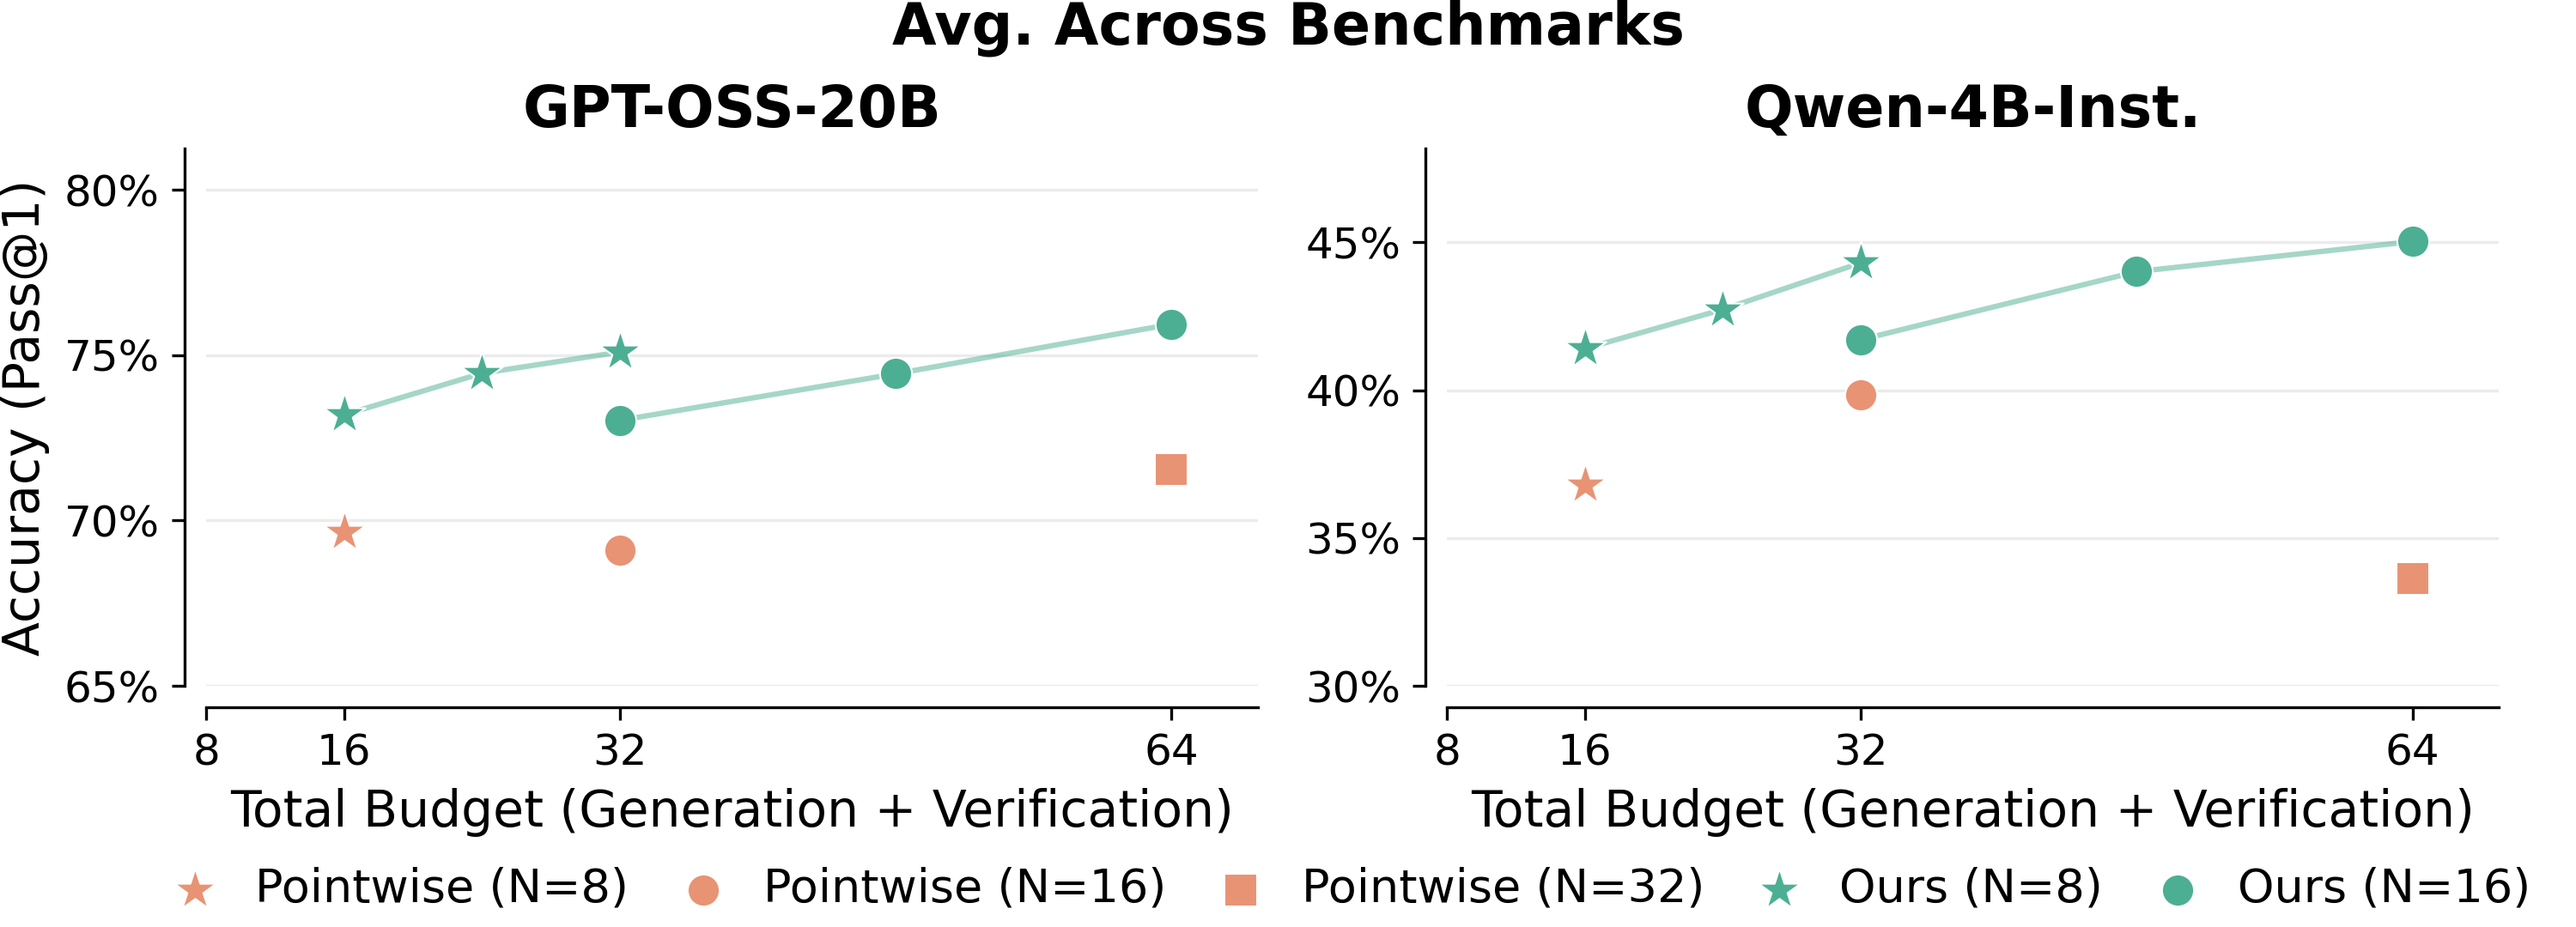
\includegraphics[width=0.85\textwidth]{images_verif/budget_vs_accuracy_avg_manual.png}
    \caption{
        Accuracy vs. total budget (generation + verification calls). Stars, circles, and squares denote $N=8$, $N=16$, and $N=32$ base generations from the LLM, while the total budget $= N + V$ where V is the number of verification calls. \pairinfer{} consistently outperforms pointwise self-verification at equivalent budgets and shows monotonic performance scaling with compute. See Fig.~\ref{fig:appendix_budget_per_benchmark} for per-benchmark results.
    }
    \label{fig:budget-accuracy}
\end{figure}

\begin{figure}[H]
    \centering
    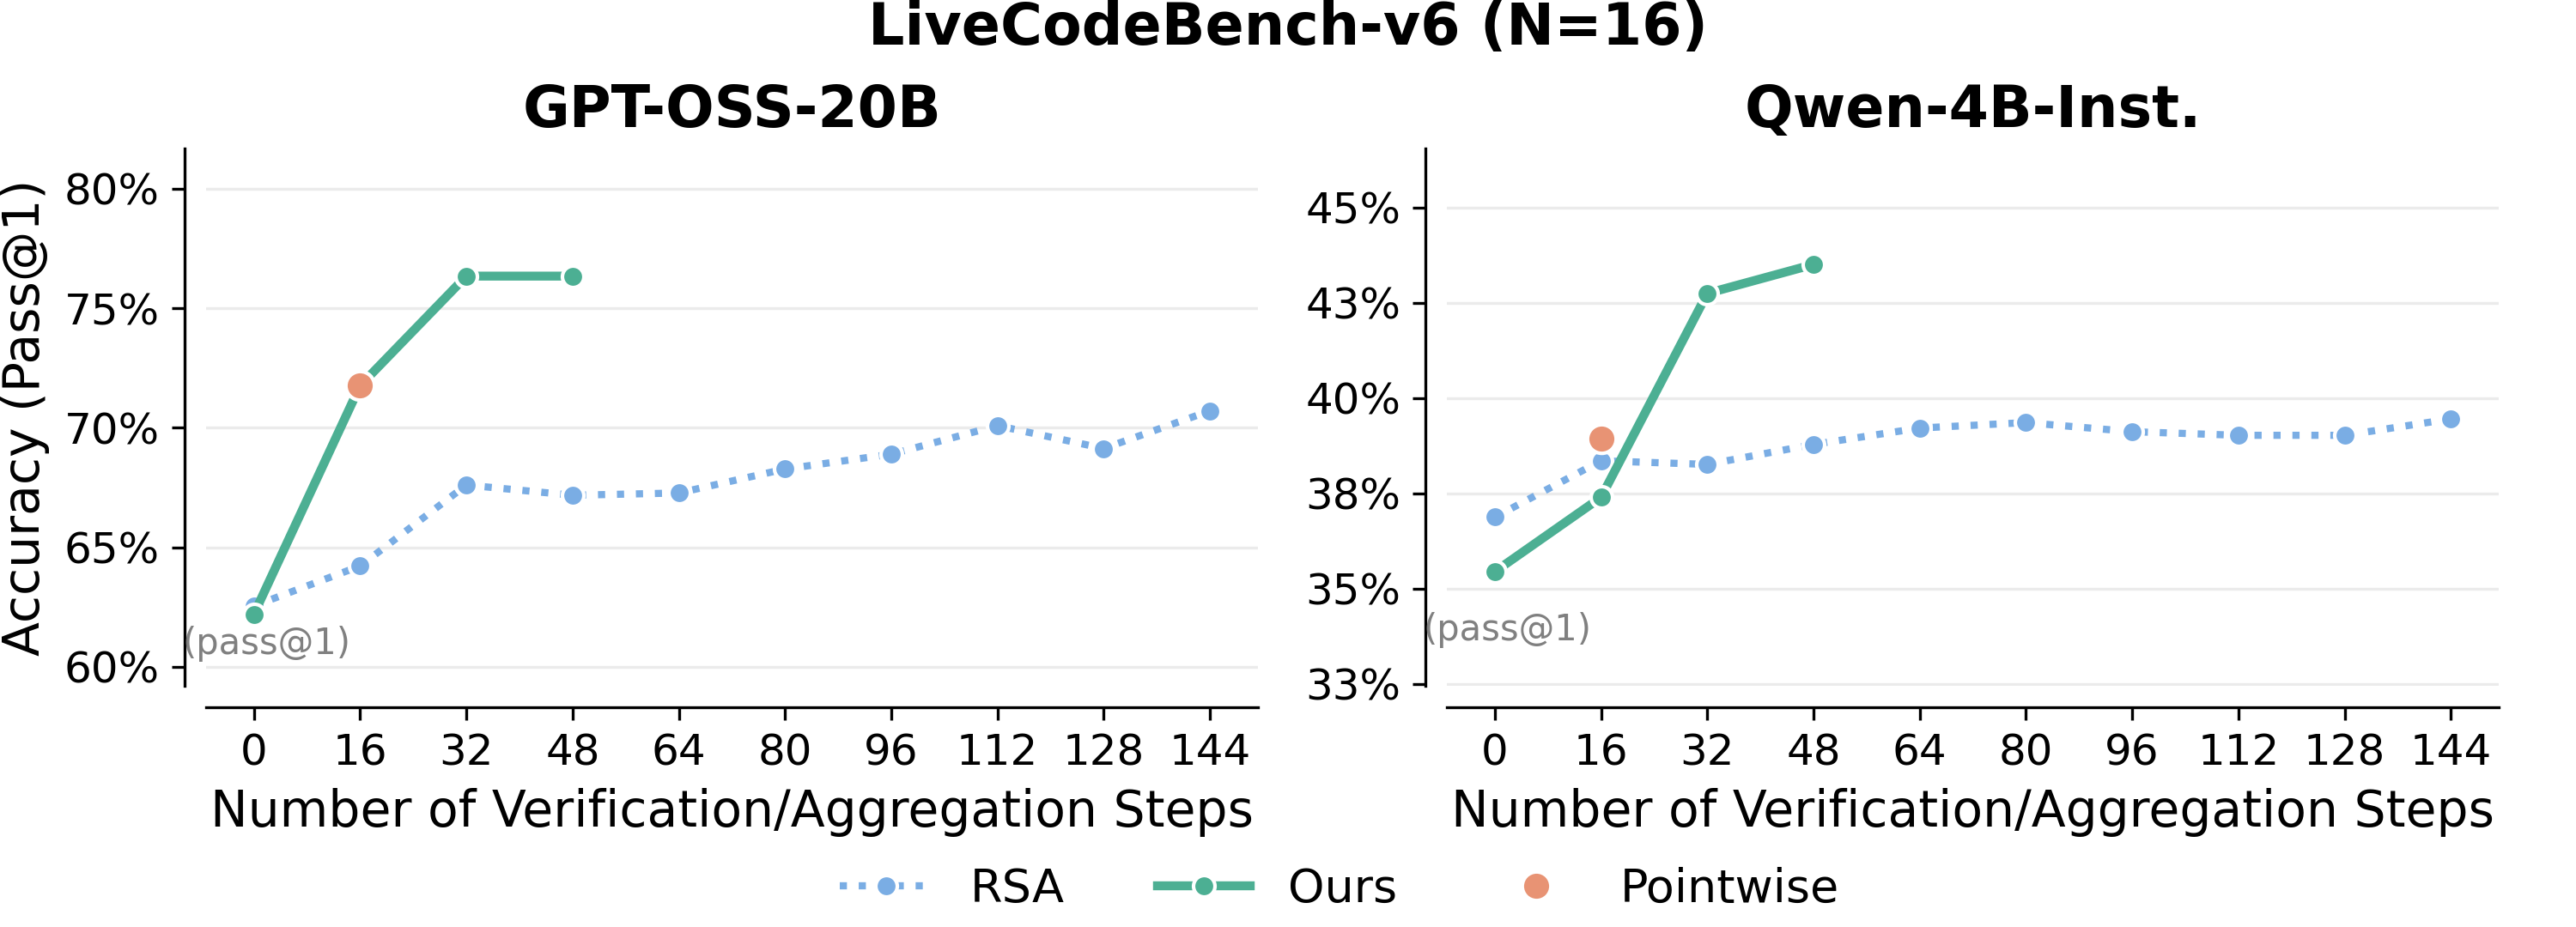
\includegraphics[width=0.85\textwidth]{images_verif/LiveCodeBench-v6_Combined_N16_LLMCalls_Comparison.png}
    \caption{
        Comparison with Recursive Self-Aggregation (RSA) \citep{venkatraman2025recursiveselfaggregationunlocksdeep} on LCB-v6. \pairinfer{} achieves higher accuracy with fewer model calls.
    }
    \label{fig:rsa-comparison}
\end{figure}


\paragraph{Uncertainty-Guided Score Aggregation.}
Standard pairwise voting often treats all ``wins'' equally, and thus fails to distinguish between a marginal preference (e.g., a 6 vs.\ 5 rating) and a decisive victory. Instead, we prompt the models to score their solutions in a pairwise setting instead of simply providing "correct" or "incorrect" as the output as in standard pairwise voting, which provides us with fine-grained information about the goodness of solutions. To capture this nuance of relative quality, we adopt a weighted aggregation scheme in which the magnitude of the rating difference serves as a proxy for the judge's confidence.
Given $N$ candidate solutions $\mathcal{S}$ generated by an LLM, and a comparison budget $B$ (number of self-verification LLM calls), a pairwise comparison between $(s_i, s_j)$ using the same LLM outputs calibrated ratings $(r_i, r_j) \in [1, 10]$ for the two solutions. We define a confidence weight
\[
w_{ij} = \max\!\left(\frac{|r_i - r_j|}{9}, \tau\right),
\]
where $\tau > 0$ is a small floor that ensures non-zero weights even for near-ties. Let $v_{ij} \in \{0, 0.5, 1\}$ denote the comparison outcome for $s_i$, corresponding to a win, tie, or loss, respectively. The estimated quality score $\mu_i$ is then computed as the uncertainty-weighted win rate
\begin{equation}
    \mu_i = \frac{\sum_{j \in \mathcal{N}(i)} w_{ij} v_{ij}}{\sum_{j \in \mathcal{N}(i)} w_{ij}},
\end{equation}
where $\mathcal{N}(i)$ denotes the set of opponents compared against $s_i$. This formulation ensures that high-confidence judgments dominate the global ranking, while ambiguous comparisons contribute minimally to score variance.

\paragraph{Phase 1: Topology Coverage.}
A primary failure mode in low-budget pairwise ranking is \textit{path dependence} in which solutions become ``orphaned'' or misranked due to insufficient pairwise comparisons with other solutions. We mitigate this by enforcing a minimum degree constraint to ensure all solutions are pairwise self-verified at least a minimum number of times. We begin with random disjoint pairings to guarantee global connectivity ($d_i \ge 1$), ensuring every solution enters the tournament. Subsequently, we iteratively target under-sampled nodes ($d_i < d_{\min}$) to meet a minimum degree threshold. Rather than selecting random opponents, we pair these low-degree nodes with candidates having the closest current mean score $\mu$. This ``anchors'' solutions against comparable peers early in the process, preventing initial noise from propagating into the refinement phase.

\paragraph{Phase 2: Swiss Refinement.}
With the topology anchored, the remaining budget focuses on resolving rank ambiguity through an uncertainty-aware Swiss system. In each round, solutions are sorted by their current score $\mu$, and we pair neighbors within a local window to minimize the score gap $|\mu_i - \mu_j|$ among unseen pairs. This strategy is grounded in active learning principles: under Bradley-Terry models, comparisons between items of similar skill (near-ties) yield the highest marginal information gain. By concentrating the judge budget on these ambiguous decision boundaries, \pairinfer{} efficiently reduces uncertainty where it matters most, achieving high ranking accuracy even with a sparse comparison graph ($K \ll N$). See Appendix \S\ref{sec:appendix_algo} for the detailed algorithm and full specification of the helper procedures.


\begin{algorithm}[t]
\caption{Uncertainty-Guided Pairwise Ranking}
\label{alg:ugpr}
\footnotesize
\begin{algorithmic}[1]
\Require Problem $x$, candidates $\mathcal{S}=\{s_i\}_{i=1}^N$, pairwise budget $B$,
min-degree $d_{\min}$, Swiss window size $h$, weight floor $\tau$
\Ensure Ranking $\pi$

\State \textbf{Initialize:} $\forall$ $i$, scores $\mu_i \gets 0.5$ and degrees $d_i\gets 0$
\State \hspace{1.0em} history $\mathcal{H}\gets\emptyset$ \Comment{$(i,j)\in\mathcal{H}$ iff $(s_i,s_j)$ has been compared}
\State \hspace{1.0em} state $\mathcal{T}\gets (\{\mu_i\}_{i=1}^N,\{d_i\}_{i=1}^N,\mathcal{H})$
\State used $\gets 0$

\Statex \textbf{Phase 1: Topology Coverage}
\While{used $< B$ \textbf{and} $\exists i : d_i < d_{\min}$}
    \State $\mathcal{P} \gets \Call{CoveragePairs}{\mathcal{T}, d_{\min}}$
    \State $\mathcal{O} \gets \Call{PairSelfVerify}{x,\mathcal{S},\mathcal{P}}$ \Comment{parallel LLM judging}
    \State $\Call{UpdateStats}{\mathcal{T}, \mathcal{O}, \tau}$ \Comment{update $\mu_i$, $d_i$; record $\mathcal{H}$}
    \State used $\gets$ used $+|\mathcal{P}|$
\EndWhile

\Statex \textbf{Phase 2: Swiss Refinement}
\While{used $< B$ \textbf{and} $N>2$}
    \State $\pi \gets \Call{Rank}{\{\mu_i\}_{i=1}^N}$ \Comment{descending $\mu$}
    \State $\mathcal{P} \gets \Call{SwissPairs}{\pi, \mathcal{T}, h}$ \Comment{within window $h$; prefer unseen and near-ties}
    \State $\mathcal{O} \gets \Call{PairSelfVerify}{x,\mathcal{S},\mathcal{P}}$
    \State $\Call{UpdateStats}{\mathcal{T}, \mathcal{O}, \tau}$
    \State used $\gets$ used $+|\mathcal{P}|$
\EndWhile

\State \Return $\Call{Rank}{\{\mu_i\}_{i=1}^N}$
\end{algorithmic}
\end{algorithm}


\subsection{Experimental Settings}

\textbf{Models and Benchmarks.} We evaluate four diverse models: GPT-OSS-20B, Qwen3-4B-Instruct, GPT-OSS-120B, and Qwen3-4B-Thinking. For code generation, we use LiveCodeBench-v5 (279 problems between date range of 24.08 to 25.02), LiveCodeBench-v6 (131 problems between 25.02-25.05 following official Qwen3-2507 models\footnote{\hyperlink{https://huggingface.co/Qwen/Qwen3-4B-Instruct-2507}{https://huggingface.co/Qwen/Qwen3-4B-Instruct-2507}})~\citep{jain2024livecodebench}, and CodeContests (165 problems)~\citep{li2022codecontests}. For real-world software engineering, we evaluate on SWE-bench Lite~\citep{jimenez2024swebench} (300 instances) using Gemini-2.5-Flash~\citep{comanici2025gemini25} as both the generation and verification model. For math, we use AIME'25 and HMMT'25~\citep{balunovic_srimatharena_2025}.

\textbf{Evaluation Protocol and Baselines.} For all methods, we first generate $N$ candidate solutions independently from the model, then apply the verification strategy to select the final answer. We use $N \in \{8, 16\}$ for most experiments, and additionally $N=32$ for pointwise verification in budget-matched comparisons. For comparison with RSA~\citep{venkatraman2025recursiveselfaggregationunlocksdeep} we keep the population size as $N=16$ with $k=4$ as the aggregation size (number of solutions to aggregate at a time), with $T=10$ RSA steps (number of recursive steps that the RSA algorithm is run for). See \citet{venkatraman2025recursiveselfaggregationunlocksdeep} for a detailed explanation of these parameters. Details about the parameters and settings for inference sampling and swiss-refinement algorithm are provided in Appendix~\ref{sec:appendix_hyperparams}.

\textbf{Pointwise Baseline.} For fair comparison, pointwise self-verification uses the same 1--10 grading system as our pairwise method. The model evaluates each solution in isolation by assigning a score between 1 and 10, and the solution with the highest score is selected. This ensures that any performance differences stem from the pairwise comparison structure rather than the scoring mechanism. The exact prompts for both pointwise and pairwise verification (for code and math) are provided in Appendix~\ref{sec:appendix_prompts}.

\textbf{Verification Budget.} \pairinfer{} allows flexible control over the verification budget. We report results for budget multipliers of 1$\times$, 2$\times$, and 3$\times$ the number of initially generated solutions ($N$). For example, with $N=16$ and budget 2$\times$, we perform 32 pairwise comparisons.


\subsection{Results}

Our goal is to measure the efficacy of \pairinfer{} compared to standard LLM-as-a-judge (pointwise) verification for parallel reasoners, and analyze how it compares with pointwise and aggregation-based test-time scaling methods in a budget-matched setting. Figures~\ref{fig:inference-results}, \ref{fig:budget-accuracy}, and \ref{fig:rsa-comparison} provide an overview of our results, comparing pointwise verification with pairwise verification (Figure~\ref{fig:inference-results}), budget-matched evaluation (Figure~\ref{fig:budget-accuracy}), and budgeted comparison with Recursive Self-Aggregation (Figure~\ref{fig:rsa-comparison}).

\textbf{\pairinfer{} consistently outperforms pointwise self-verification.}
On CodeContests, GPT-OSS-20B improves from 66.06\% to 73.33\% (+7.3\%), while Qwen3-4B-Instruct improves from 39.4\% to 46.1\% (+6.7\%). On LiveCodeBench-v5, GPT-OSS-20B gains +8.6\% and Qwen3-4B-Instruct gains +4.3\%. On HMMT, GPT-OSS-20B gains +10.0\% and Qwen3-4B-Instruct gains +6.7\%. See Figure~\ref{fig:inference-results} for more results and Appendix Figure~\ref{fig:appendix-all-verif-bars} for results on Qwen-4b-Thinking-2507 and GPT-OSS-120B. These results demonstrate that pairwise comparisons provide more informative signals than independent pointwise scores. We further observe that as verification budget increases, pairwise verification performance improves or stays consistent across most models and benchmarks (see Appendix Figure~\ref{fig:appendix-all-verif-bars}). While the results above are for the same number of base solution generations (N=16), we find similar trends while comparing methods in a compute-matched setting as well, Figure~\ref{fig:budget-accuracy}, e.g., with a compute budget of 64 model calls, with Qwen3-4B-Instruct-2507, pointwise verification performs approx. 33\% while pairwise verification reaches 45\% accuracy on average on code gen. benchmarks.


\textbf{\pairinfer{} enables improved test-time scaling.} We compare against Recursive Self-Aggregation (RSA)~\citep{venkatraman2025recursiveselfaggregationunlocksdeep}, a state-of-the-art test-time scaling method that iteratively refines solutions through an evolutionary self-aggregation process. As shown in Figure~\ref{fig:rsa-comparison}, \pairinfer{} achieves higher accuracy with significantly fewer LLM calls. On LiveCodeBench-v6 with N=16, our method reaches 76\% Pass@1 with only 48 verification calls, higher compared to the maximum accuracy attained by RSA. This efficiency stems from our uncertainty-guided Swiss refinement, which concentrates comparisons on informative pairs rather than exhaustively aggregating or verifying all solution pairs. See Figures.  \ref{fig:appendix_lcb_all_models_16}, \ref{fig:appendix_lcb_all_models_8}, \ref{fig:appendix_budget_per_benchmark} for extended results.

\begin{wrapfigure}{r}{0.57\textwidth}
  \centering
  \vspace{-1em}
  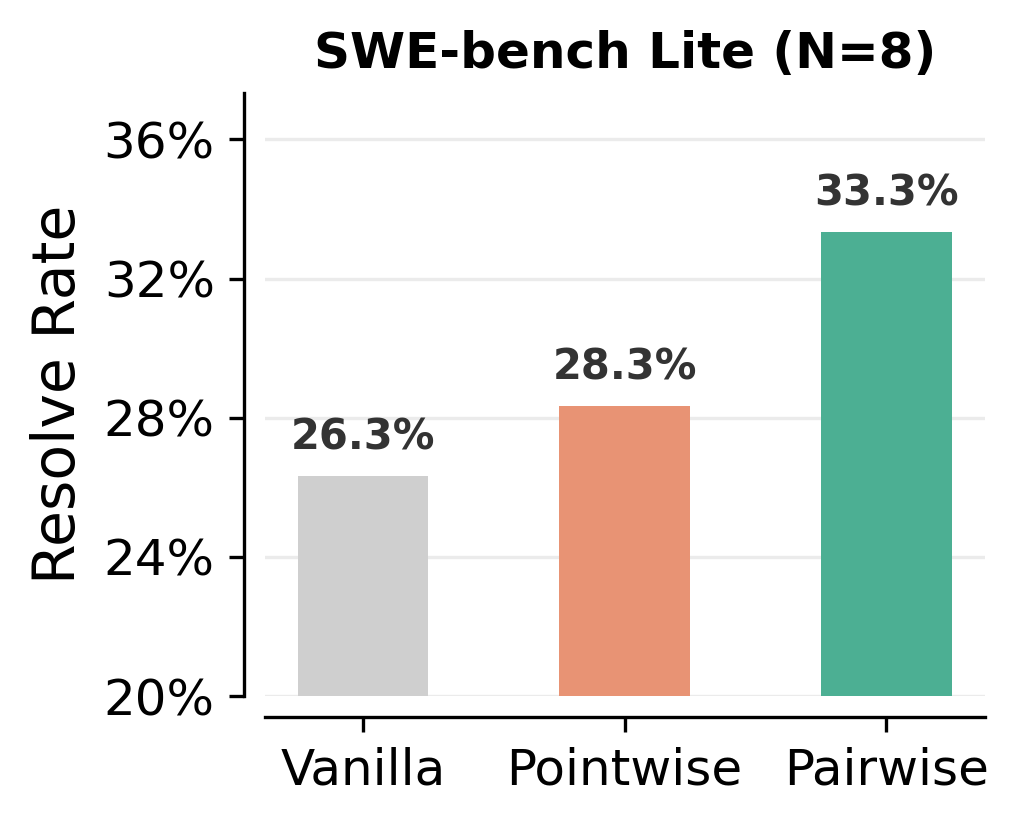
\includegraphics[width=0.55\textwidth]{images_verif/swe_bench_lite_verification.png}
  \caption{Pairwise comparison with vanilla solution generation and pointwise self-verification on SWE-bench Lite (300 instances, $N{=}8$ candidates, Gemini 2.5 Flash, mini-swe-agent~\citep{yang2024sweagent} pipeline).}
  \label{fig:swe_bench_results}
  \vspace{-1em}
\end{wrapfigure}
\textbf{Generalization to real-world software engineering tasks.} To evaluate whether pairwise self-verification extends beyond competitive programming and math to open-ended software engineering, we apply \pairinfer{} to SWE-bench Lite~\citep{jimenez2024swebench}, a benchmark of 300 real GitHub issues from popular Python repositories. For each instance, we use Gemini-2.5-Flash to generate $N{=}8$ candidate patches via an agentic coding pipeline (mini-swe-agent~\citep{yang2024sweagent}), then apply self-verification to select the final patch. Crucially, the verification step receives \emph{only} the issue description and the candidate patch diffs. No repository context, execution feedback, or agent trajectory is provided, making this a pure self-verification setting. As shown in Figure~\ref{fig:swe_bench_results}, pairwise verification achieves a 33.3\% resolve rate compared to 28.3\% for pointwise and 26.3\% for vanilla (first-candidate) selection, an absolute gain of +5.0\% over pointwise and +7.0\% over vanilla. This result demonstrates that head-to-head patch comparison enables the verifier to identify subtle correctness differences, such as proper root-cause fixes versus surface-level changes, that are difficult to assess in isolation. See Appendix~\ref{sec:appendix_swe_examples} for detailed examples showing how pairwise and pointwise verification select different patches across diverse bug categories.

\clearpage
\subsection{Analysis and Ablations}

\begin{wrapfigure}{r}{0.41\textwidth}
  \centering
  \vspace{-1.5em}
  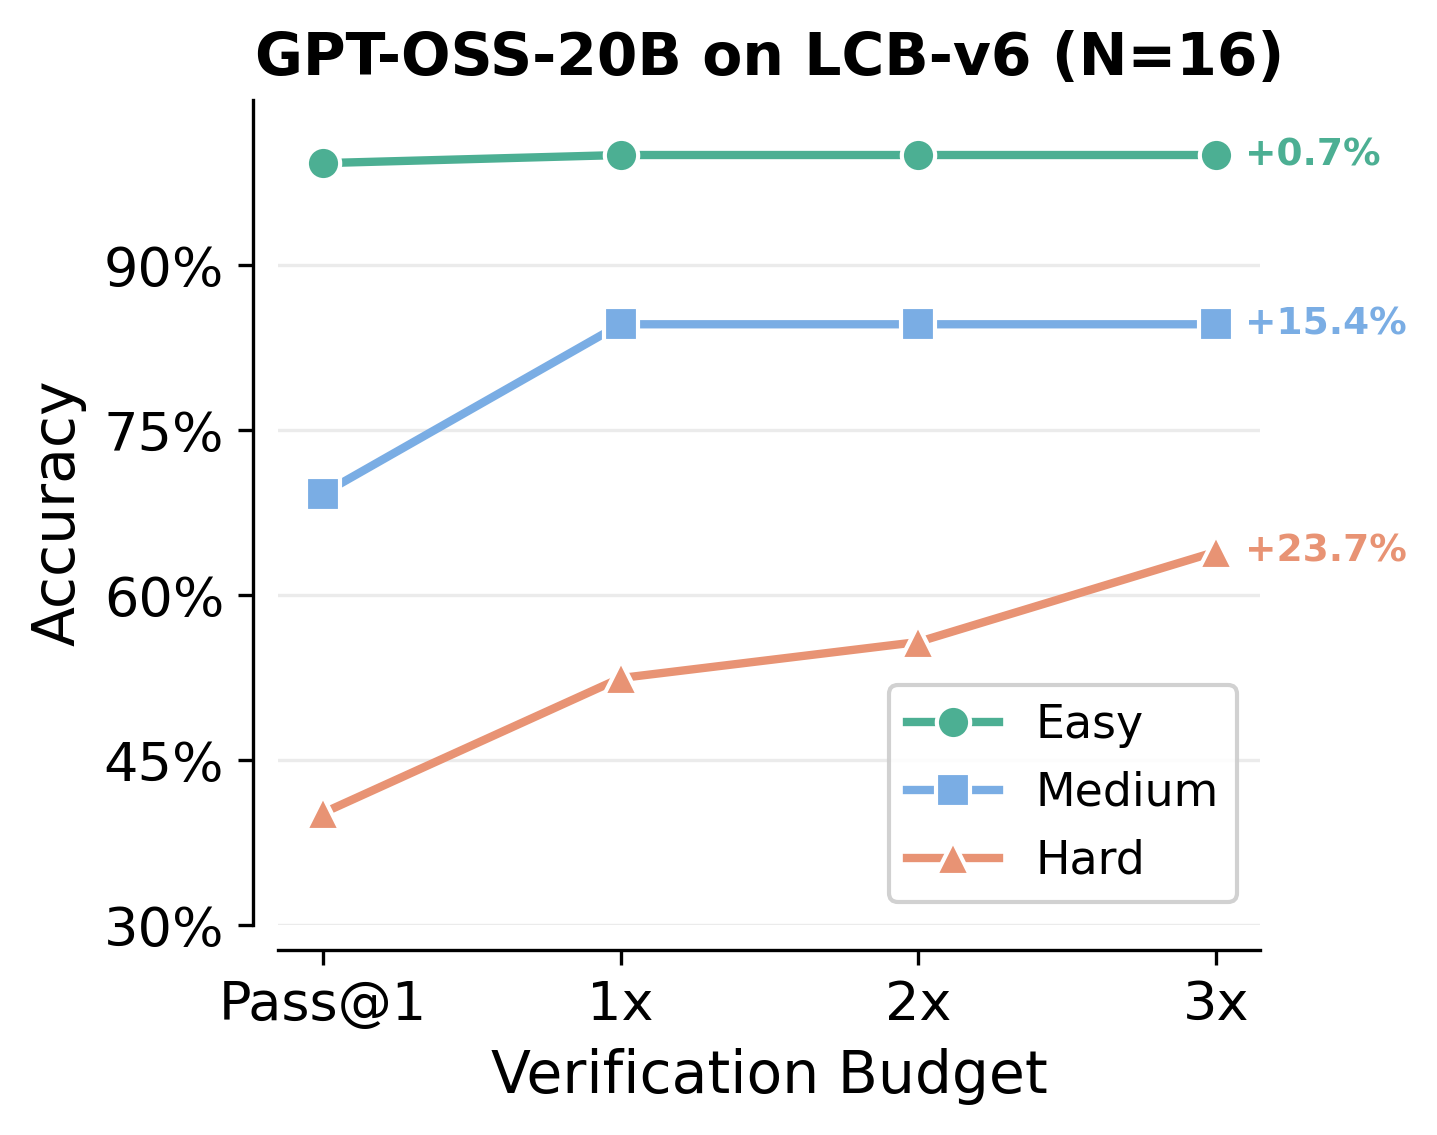
\includegraphics[width=0.43\textwidth]{images_verif/difficulty_verification_trajectory.png}
  \caption{Accuracy improvement with increasing verification budget across problem difficulty levels (GPT-OSS-20B on LCB-v6, N=16). \pairinfer{} provides the largest gains on hard problems (+23.7\%).}
  \label{fig:difficulty_trajectory}
  \vspace{-1em}
\end{wrapfigure}
\textbf{Performance gains across different difficulty levels.} Figure~\ref{fig:difficulty_trajectory} shows how \pairinfer{} improves accuracy across different problem difficulty levels. On easy problems, Pass@1 is already near-optimal (99.3\%). However, on hard problems where Pass@1 is only 40.2\%, pairwise verification with budget 3x achieves 63.9\%, a gain of +23.7\%. Medium difficulty problems show an improvement of +15.4\%. This pattern demonstrates that \pairinfer{} is most valuable precisely where it is needed most: on challenging problems where the model generates a diverse set of candidate solutions and accurate selection among them is critical for bridging the gap between Pass@1 and Pass@N.

\textbf{\pairinfer{} outperforms random pairwise verification.} To validate the effectiveness of our uncertainty-guided refinement algorithm, we compare against a baseline that randomly selects pairs for pairwise comparison. On LCB-v6 with GPT-OSS-20B at budget 3$\times$, \pairinfer{} achieves 76.3\% accuracy compared to 72.5\% for random pairing, a gain of +3.8\%. This demonstrates that the strategic pair selection in \pairinfer{}, which prioritizes comparisons between solutions with similar quality scores, yields more informative judgments than random sampling.

\begin{wrapfigure}{r}{0.41\textwidth}
  \centering
  \vspace{-1.5em}
  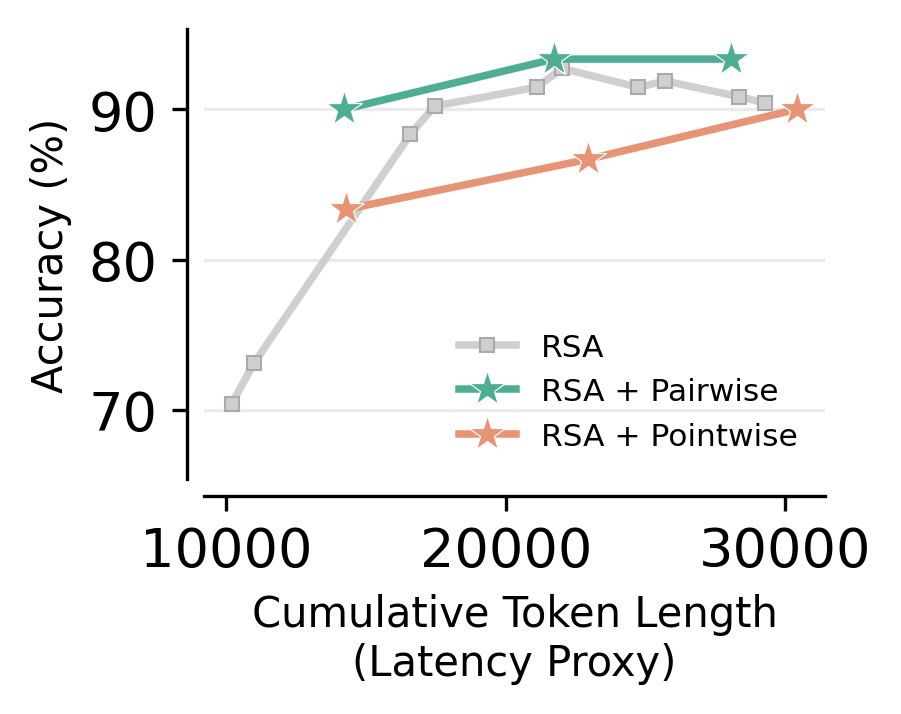
\includegraphics[width=0.43\textwidth]{images_verif/rsa_verif_combined_aime.png}
  \caption{Combining self-verification with RSA on AIME 2025.}
  \label{fig:rsa_verif_combined}
  \vspace{-1em}
\end{wrapfigure}
\textbf{Complementing aggregation with self-verification for better test-time scaling.} Self-verification and aggregation-based approaches such as RSA~\citep{venkatraman2025recursiveselfaggregationunlocksdeep} offer complementary benefits for test-time scaling. RSA is verifier-free, relying on implicit verification through iterative self-aggregation, while evolutionary approaches like AlphaEvolve~\citep{novikov2025alphaevolve} depend on external evaluators to guide search. By combining aggregation with pairwise self-verification, the model's own verification capability can serve as an explicit fitness signal within the evolutionary loop. We explore this by running RSA with population size $N{=}16$ and aggregation size $k{=}4$: every 2 RSA loops, we apply self-verification to the 16 candidates, retain the top 8 by verification score, construct 16 new aggregation sets of 4 from these 8, and continue the RSA loop to maintain the population size. As shown in Figure~\ref{fig:rsa_verif_combined}, pairwise self-verification reaches 90\% accuracy early in the RSA loop and converges to 93.3\% with lower cumulative latency than vanilla RSA requires to reach comparable accuracy. In contrast, pointwise self-verification converges more slowly, lagging behind both pairwise and vanilla RSA at equivalent latency. This demonstrates that pairwise self-verification provides a reliable fitness signal for guiding evolutionary test-time scaling, enabling improved convergence with fewer aggregation steps.


\textbf{Qualitative analysis: why pairwise outperforms pointwise on code.} We examine representative LCB-v6 problems where pairwise and pointwise verification select different solutions (Qwen3-4B-Instruct, N=16; full examples in Appendix~\ref{sec:appendix_code_examples}). A recurring failure mode of pointwise verification is \emph{score saturation}: the verifier assigns high scores (e.g., 10/10) to most candidates, losing its ability to discriminate. These patterns suggest that pairwise comparison provides a natural calibration mechanism: instead of assigning an absolute quality score, the verifier only needs to determine which of two solutions is better, a judgment that is more robust than absolute rating. We illustrate two representative cases below.

\begin{tcolorbox}[
    colback=blue!2,
    colframe=blue!15,
    breakable,
    enhanced
]
\small
\textbf{Example 1: Group Element Assignment (4/16 correct). Pairwise \checkmark, Pointwise \ding{55}.}
Assign elements to groups by divisibility (smallest index wins).
Pointwise assigns 12 of 16 candidates the maximum score 10/10, selecting an $O(|\text{groups}| {\times} |\text{elements}|)$ brute-force that passes examples but exceeds time limits on large inputs. Pairwise ($\mu{=}0.917$) selects a solution using divisor enumeration ($O(\sqrt{g})$ per group) with a hash map. Head-to-head comparison surfaces the algorithmic difference that independent scoring misses.

\vspace{0.5em}
\textbf{Example 2: Binary String Trade (1/16 correct). Pairwise \checkmark, Pointwise \ding{55}.}
Maximize active sections after at most one trade on an augmented binary string.
Only 1 of 16 solutions is correct (idx=15). Pointwise gives it 8/10 but gives an incorrect solution (idx=4) the maximum 10/10. Pairwise assigns the correct solution the highest $\mu$ score of 1.000 through head-to-head wins, successfully finding the needle in a haystack of 16 candidates.

\vspace{0.3em}
{\footnotesize See Appendix~\ref{sec:appendix_code_examples} for full code and additional examples.}
\end{tcolorbox}

\begin{tcolorbox}[title=Takeaway: Improved Self-Verification and Test-Time Scaling with \pairinfer{}, colback=green!5]
Pairwise self-verification (\pairinfer{}) yields more accurate candidate ranking than pointwise scoring and enables improved performance by test-time scaling of verification compute, compared with self-aggregation based test-time scaling. Furthermore, pairwise self-verification is complementary to aggregation-based approaches: when combined with RSA, it improves convergence latency by providing a reliable fitness signal within the evolutionary loop.
\end{tcolorbox}


\section{\method{}-PairRL: Improving Self-Verification via Unified RL Training}
\label{sec:unified_rl}


The previous section demonstrated that pairwise self-verification significantly outperforms pointwise approaches at inference time.
In the remainder of the paper we consider a second question: \textit{can we explicitly train models to become stronger self-verifiers?} Current RL paradigms for reasoning focus almost exclusively on optimizing the generation of correct solutions, treating verification as either an afterthought or an external process. While recent work has explored co-training generators with verifiers \citep{sareen2025puttingvaluerlbetter, liu2025trustverifyselfverificationapproach}, these approaches rely on \textit{pointwise} rewards and fail to leverage the parallel responses that techniques like GRPO naturally generate during training. Additionally, pointwise verification is uncalibrated, which may make optimization hard. Other methods train for aggregation awareness \citep{venkatraman2025recursiveselfaggregationunlocksdeep, zhao2025majority} but use offline data, limiting the model's ability to adapt to its own evolving generation distribution during RLVR training.

We propose \method{}-PairRL, a unified RL framework that trains a single LLM to be both a strong reasoner and an accurate \textit{pairwise} self-verifier. The key insight is that generation and verification should \textit{co-evolve}: as the generator improves, the distribution of responses changes, and the verifier must learn score increasingly high-quality solutions. This online, co-evolving setup ensures verification training data is always in-distribution for the model's current capabilities. However, unified training introduces unique challenges: naive implementations suffer from reward hacking, where the generator and verifier collude to maximize reward without improving actual capabilities. We address these challenges through careful reward design and pairing strategies.

\begin{figure}[t]
    \centering
    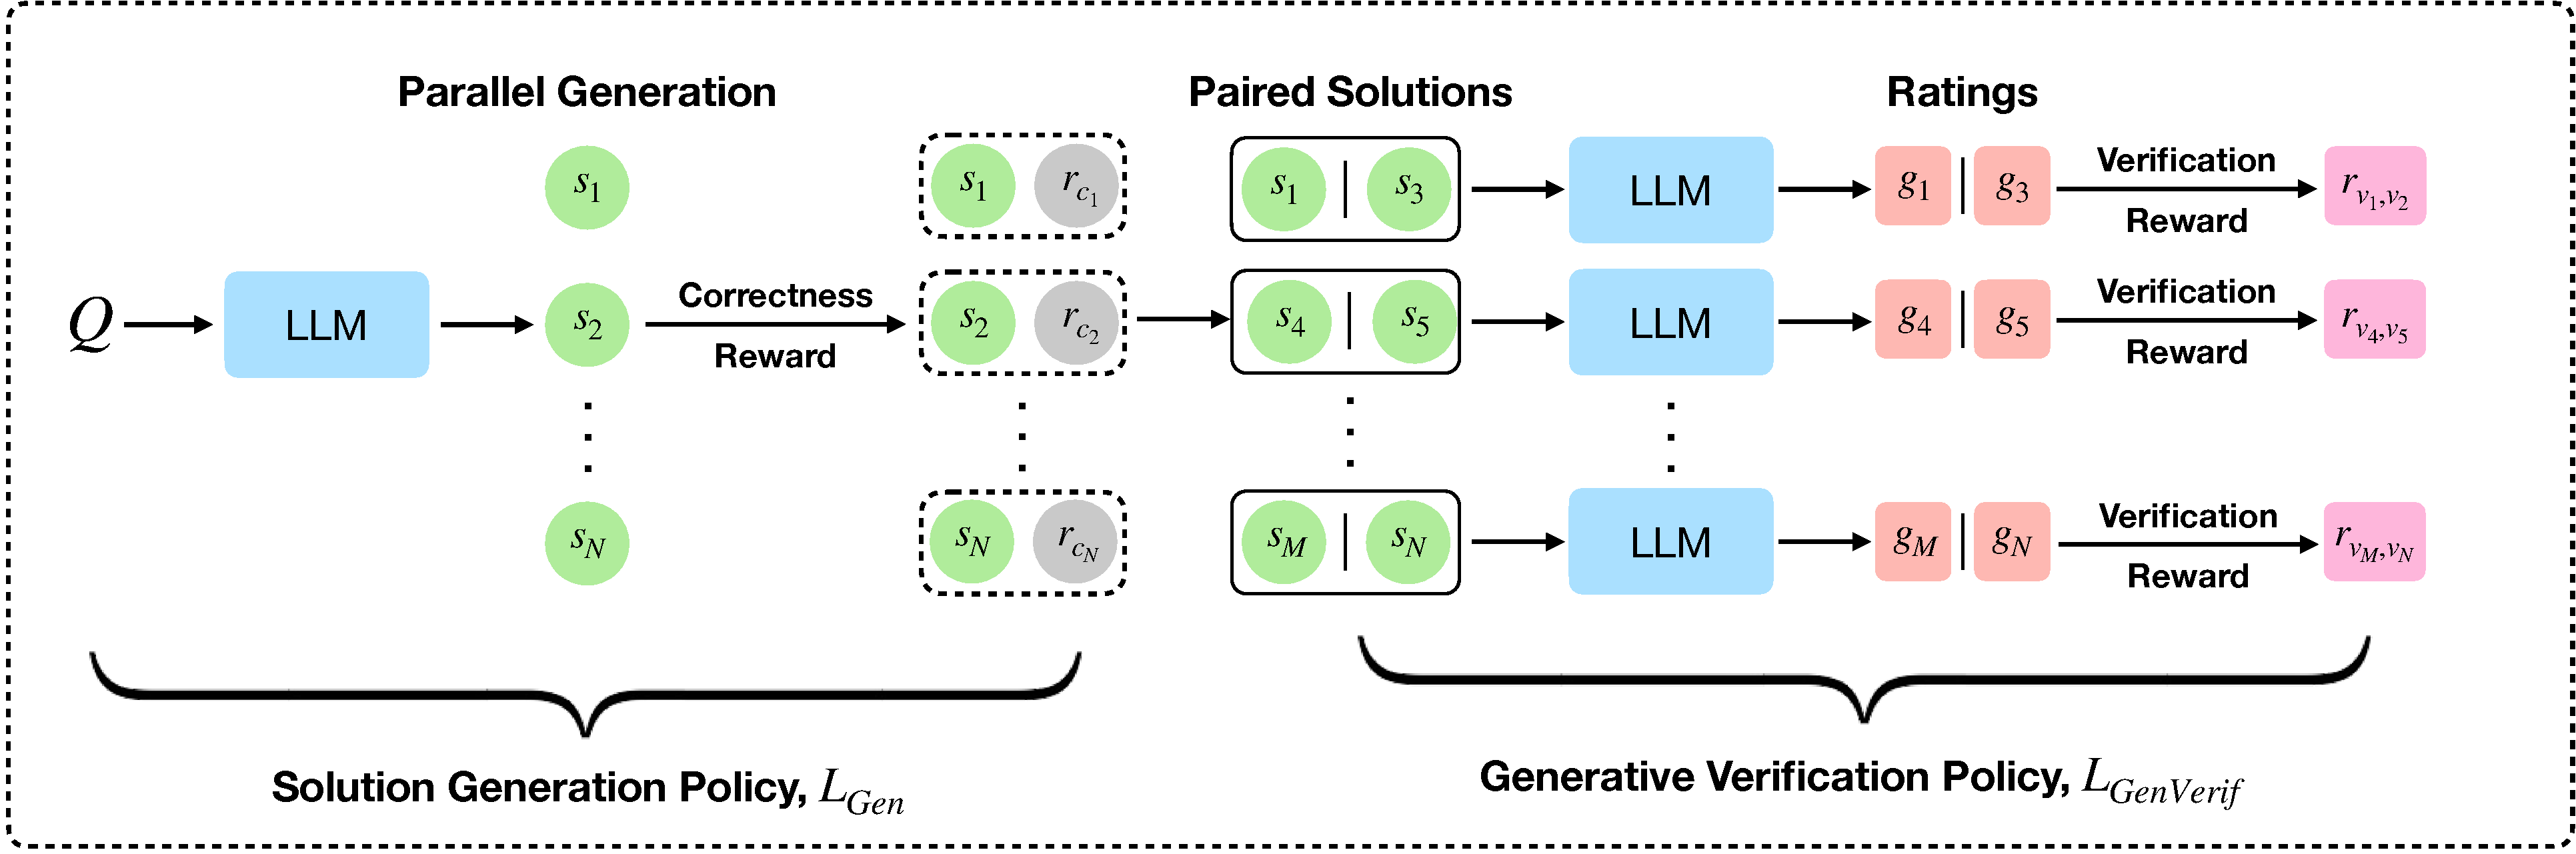
\includegraphics[width=0.9\textwidth]{figures/fig_2_plot_rl_ver.pdf}
    \caption{\textbf{\method{}-PairRL: Unified RL training for co-evolving generation and pairwise verification.} A single LLM is trained with two objectives: $J_{\text{Gen}}$ optimizes solution generation using correctness rewards, while $J_{\text{PairVerif}}$ optimizes pairwise verification accuracy. The generator produces $G$ solutions per problem, which are evaluated for correctness and paired for verification training. The verifier evaluates solutions in a paired setting by providing correctness scores for both solutions. Since we are in a verifiable setting and know from ground truth (such as test case execution during code generation) which of the generator solutions are correct, we can calculate correctness rewards for the verifier as well. See Section~\ref{sec:unified_rl} for more details on how optimization proceeds and rewards are calculated in this framework.}
    \label{fig:unified_rl_overview}
\end{figure}

\subsection{Preliminaries: RL for LLMs}
The goal of RL for LLMs is to maximize expected reward $r$ of an LLM policy $\pi_\theta$ over a distribution of prompts $P(Q)$. This is commonly done with policy gradient methods. Specifically, Group-Relative Policy Optimization (GRPO) \cite{deepseekai2025deepseekr1incentivizingreasoningcapability} and its variants \cite{yu2025dapoopensourcellmreinforcement} have shown significant promise and stable optimization dynamics. In each episode, we sample prompts $q \sim P(Q)$ and a group of $G$ rollouts per prompt $ \{o_i\} \sim \pi_{\text{old}}(.|q)$. We maximize $J_{\text{Gen}}(\theta)$:
{\begin{equation} \small
    \mathop{\mathbb{E}}_{q, \{o_i\}}\left[ \frac{1}{\sum_{i=1}^G|o_i|} \sum_{i=1,t=1}^{G,|o_i|} \min \Big( \rho_{i,t} A_i, \text{clip}(\rho_{i,t}, 1\!-\!\epsilon, 1\!+\!\epsilon) A_i \Big) \right]
\end{equation}}
where $A_i = r_i - \text{mean}(\mathbf{r})$ is the advantage computed over the group and $\rho_{i,t} = \pi_\theta(o_{i,t} | q, o_{i,<t}) / \pi_{\text{old}}(o_{i,t} | q, o_{i,<t})$ is the importance sampling ratio.

\subsection{Co-evolving Solver-Verifier Training}
Our training objective combines generation and pairwise verification in a unified RL formulation:
\begin{equation}
    J(\theta) = J_{\text{Gen}}(\theta) + \lambda J_{\text{PairVerif}}(\theta)
\end{equation}
$J_{\text{Gen}}$ optimizes the likelihood of correct reasoning paths (using GRPO) and $J_{\text{PairVerif}}$ optimizes the accuracy of pairwise ranking judgments. Both objectives use the \textit{same} rollouts: during each training step, the model generates $G$ solutions per problem, which are used both to compute generation rewards and to form solution pairs for verification training.
This ensures the verifier always trains on in-distribution data from the current policy. For verification training, we do one LLM call for each input pair of solutions. Figure~\ref{fig:unified_rl_overview} shows an overview of \method{}-PairRL. While our framework is general, we instantiate experiments on RL for code-generation following DeepCoder \citep{deepcoder2025}.

\textbf{Rewards.}
For the solution generator, we use a standard binary correctness reward $r_{\text{gen}} \in \{0, 1\}$ based on passing all ground truth test cases. Reward is set to 0 if response formatting is incorrect, i.e., the model does not output the response withing thinking tags as mentioned in the prompt (\S\ref{sec:generation_prompts}). For the pairwise self-verification objective, the model compares two solutions $(s_A, s_B)$ and outputs a confidence score between 1 and 10, which is normalized to $v_i \in [0, 1]$ for each solution. We reward the verifier based on how well its scores align with ground truth correctness $y_i \in \{0, 1\}$:
\begin{equation}
    r_{\text{verif}} = \frac{1}{2} \sum_{i \in \{A, B\}} \mathbb{I}(|v_i - y_i| \leq 0.2) \cdot (1 - |v_i - y_i|)
\end{equation}
The indicator function $\mathbb{I}(|v_i - y_i| \leq 0.2)$ implements a \textit{sparsity threshold}: the verifier receives reward only when its score is within 0.2 of the ground truth (i.e., scoring a correct solution $\geq 0.8$ or an incorrect solution $\leq 0.2$). This design choice is critical for preventing reward hacking, which we discuss below.


\begin{figure}[t]
  \centering
  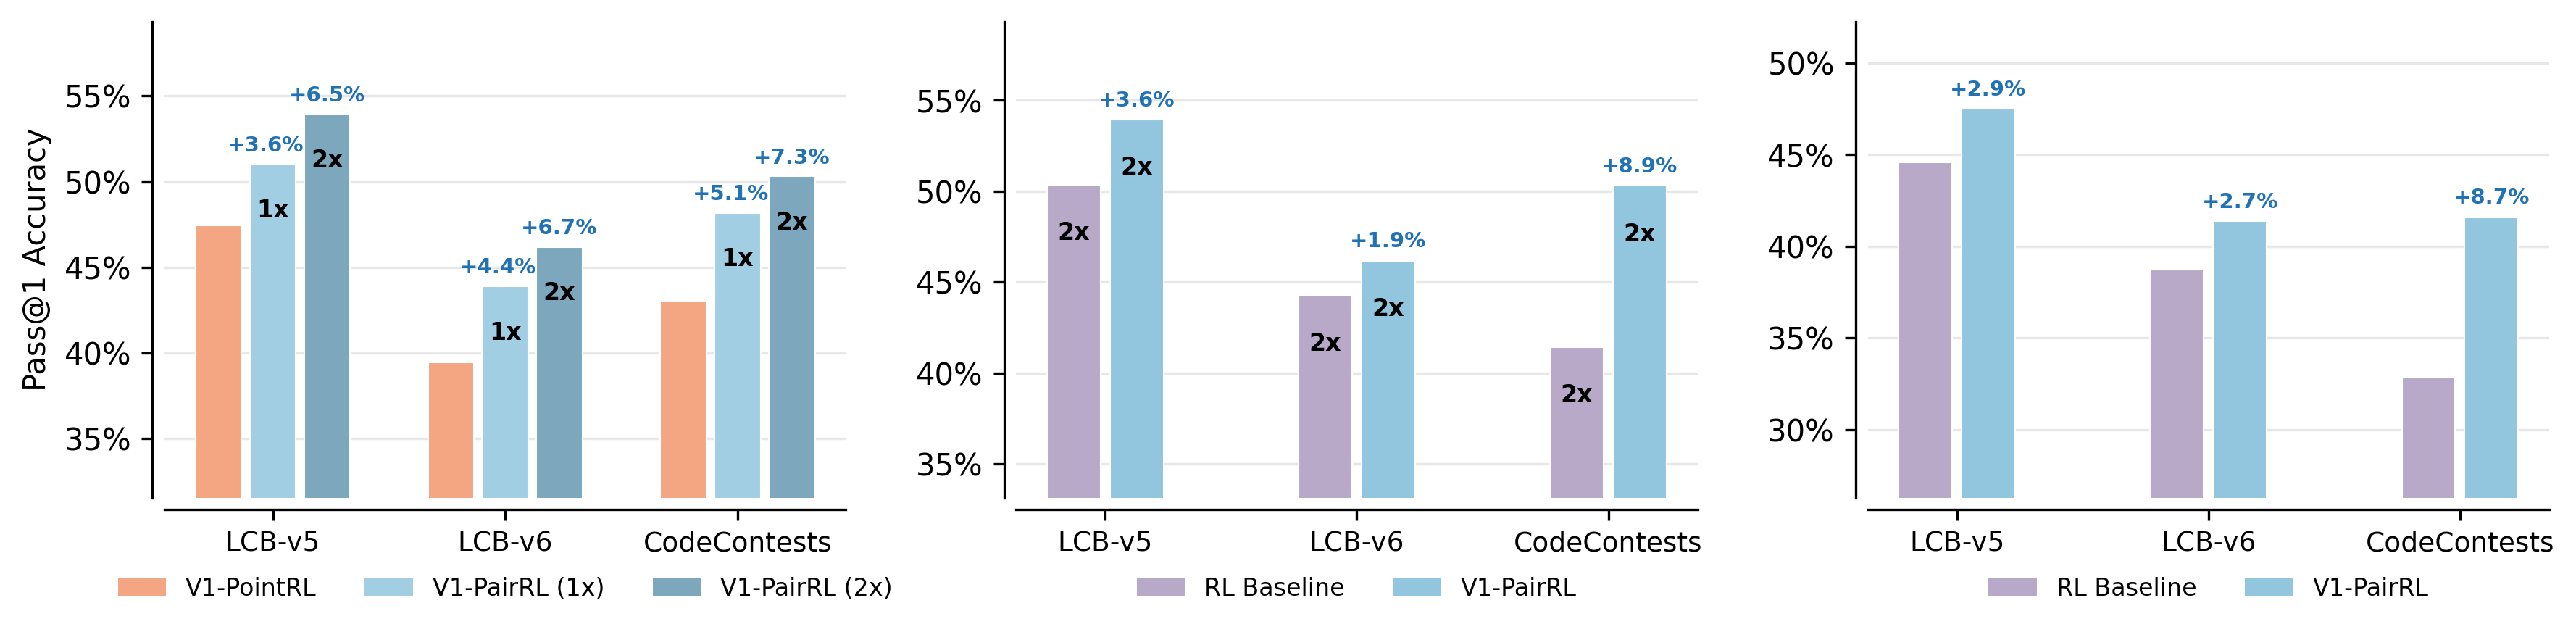
\includegraphics[width=0.95\textwidth]{images_verif/TrainedModels_Combined_Panel_N16.png}
  \caption{\textbf{\method{}-PairRL training results (N=16).}
  \textbf{(left)} Test-time scaling: \method{}-PairRL outperforms \method{}-PointRL and improves with increased verification budget.
  \textbf{(middle)} With \pairinfer{} as the test-time scaling algorithm (at 2x budget): \method{}-PairRL outperforms RL baseline even when both use pairwise verification.
  \textbf{(right)} Base Pass@1 accuracy without any test-time scaling: Co-training with pairwise verification improves generation quality over the RL baseline, even without test time scaling.}
  \label{fig:pairv1_results}
\end{figure}


\textbf{Mitigating Reward Hacking.}
Unified training of generators and verifiers is prone to specific collapse modes. We address two critical forms of reward hacking:

1. \textit{The Safe Bet Collapse:} Without the \textbf{sparsity threshold}, the verifier learns to output a safe, middle-ground score (e.g., $v_i = 0.5$) for every solution. This minimizes the risk of being ``very wrong'' but yields a meaningless discriminator. Sparsity threshold forces the model to commit to confident judgments: only scores near 0 or 1 receive positive reward.

2. \textit{The Empty Solution Loop:} If the verifier is trained on pairs of two incorrect solutions, the generator may collapse into producing empty or trivially incorrect outputs. The verifier easily identifies these as incorrect (scoring them near 0), receiving high reward. This creates a situation where the generator degrades to maximize the verifier's ease of judgment. To prevent this, we enforce a strict pairing strategy: we only trigger verification training when we can form pairs containing at least one correct solution (Correct-Incorrect or Correct-Correct pairs).


\subsection{Experimental Settings}

We instantiate \method{} on RLVR for code generation following the DeepCoder recipe~\citep{deepcoder2025}. Models are trained on the DeepCoder training set, which comprises 24K verified coding problems, utilizing binary rewards determined by executing generated code against ground-truth test cases (1 if all pass, 0 otherwise). We track solution generation performance on the DeepCoder validation set.

\textbf{Models and Benchmarks.} We train {Qwen3-4B-Instruct-2507}, an instruction-tuned model, following the DeepCoder experimental protocol. We evaluate trained models on LiveCodeBench V5, V6, and CodeContests. See Appendix \S\ref{sec:appendix_inference_hyperparams} for evaluation hyperparameters.


\textbf{Pairwise Verification Training.} For $J_{\text{PairVerif}}$, we group multiple verification prompts (problem + solution pairs from the solver) rather than generating multiple rollouts for a single prompt. This strategy allows us to leverage information from all pairwise comparisons without increasing the total rollout budget. The advantage for verification rollouts reduces to a REINFORCE-style estimator with a mean baseline calculated across prompts.

\textbf{Baselines.} We compare our approach against two primary baselines: (1) a standard \textbf{RL baseline} trained solely for generation without a verification objective, and (2) \textbf{\method{}-PointRL}, a model jointly trained with pointwise verification rewards under the same setup. Training details for \method{}-PointRL are in App.~\ref{sec:appendix-pointwise-training}.

\textbf{Training Setup.} We adopt the DAPO~\citep{yu2025dapoopensourcellmreinforcement} configuration, removing the KL penalty, using Clip High, and applying token-level loss, and follow Dr. GRPO~\citep{liu2025understandingr1zerotraining} by removing standard deviation normalization. To ensure a fair comparison, we enforce a fixed compute budget of 8 total rollouts per problem. The baseline allocates all 8 rollouts to the solver, while co-evolving models (\method{}-PairRL and PointRL) split this budget into 4 solver and 4 verifier rollouts. We verified that training the baseline for a longer duration with fewer rollouts does not improve performance, confirming that gains stem from the co-training objective. All models are trained for 150 steps, with checkpoints selected based on the validation accuracy (pass@1). Prompts used for code-generation training are in Section~\ref{sec:generation_prompts}.

\subsection{Results}

\textbf{\method{}-PairRL Offers Superior Test-Time Scaling Capabilities.}
To evaluate the test-time scaling benefits of co-trained verification, we compare \method{}-PairRL against \method{}-PointRL, our pointwise verification baseline trained with the same co-evolving setup (as described in Appendix \ref{sec:appendix-pointwise-training}). As shown in Figure~\ref{fig:pairv1_results}(a), pairwise self-verification consistently outperforms pointwise across all benchmarks at N=16. On LiveCodeBench-v5, \method{}-PairRL achieves 53.9\% (2x budget) compared to 47.4\% for \method{}-PointRL (+6.5\%). Similar improvements are observed on LiveCodeBench-v6 (+6.8\%) and CodeContests (+7.3\%). \method{}-PairRL exhibits positive scaling with verification budget: increasing budget yields consistent accuracy gains across all benchmarks, demonstrating that the model learns to leverage additional pairwise comparisons effectively.

\textbf{\method{}-PairRL outperforms RL Baseline with \pairinfer{} as the inference algorithm.}
In a test-time scaling setup with the same algorithm, a key question arises: does \method{}-PairRL show improved performance compared to the standard RL baseline? To investigate, we apply \pairinfer{} at inference time to both \method{}-PairRL and the RL baseline, using identical 2x verification budgets. As shown in Figure~\ref{fig:pairv1_results} (middle), \method{}-PairRL consistently outperforms the RL baseline even when both leverage pairwise verification: +3.6\% on LiveCodeBench-v5, +1.9\% on LiveCodeBench-v6, and +8.9\% on CodeContests. This shows that co-training with pairwise verification enhances overall performance in an equivalent test-time scaling setup.

\textbf{\method{}-PairRL improves RL Baseline.}
Co-training for pairwise self-verification yields substantial improvements in generation quality. As shown in Figure~\ref{fig:pairv1_results}(right), \method{}-PairRL achieves consistent Pass@1 improvements over the RL baseline across all three code generation benchmarks at N=16: +2.9\% on LiveCodeBench-v5, +2.7\% on LiveCodeBench-v6, and +8.7\% on CodeContests. The gains demonstrate that jointly optimizing for generation and pairwise verification creates a beneficial learning signal that improves the model's underlying reasoning capabilities (which can also include improving the self-verification capability within long chains of thought), not just its verification accuracy. Our results echo prior findings by \citet{sareen2025puttingvaluerlbetter}, who showed that co-training with pointwise verification improves the base model's Pass@1 performance. We show that pairwise verification takes this one step further: \method{}-PairRL also outperforms \method{}-PointRL in generation quality, particularly on CodeContests (by about +6\%), where the gap is most pronounced (see Appendix Figure~\ref{fig:pairv1_vs_rl_per_benchmark}).

\subsection{Ablations}
\label{sec:analysis_ablations}
\begin{wrapfigure}{r}{0.44\textwidth}
    \centering
    \vspace{-1em}
    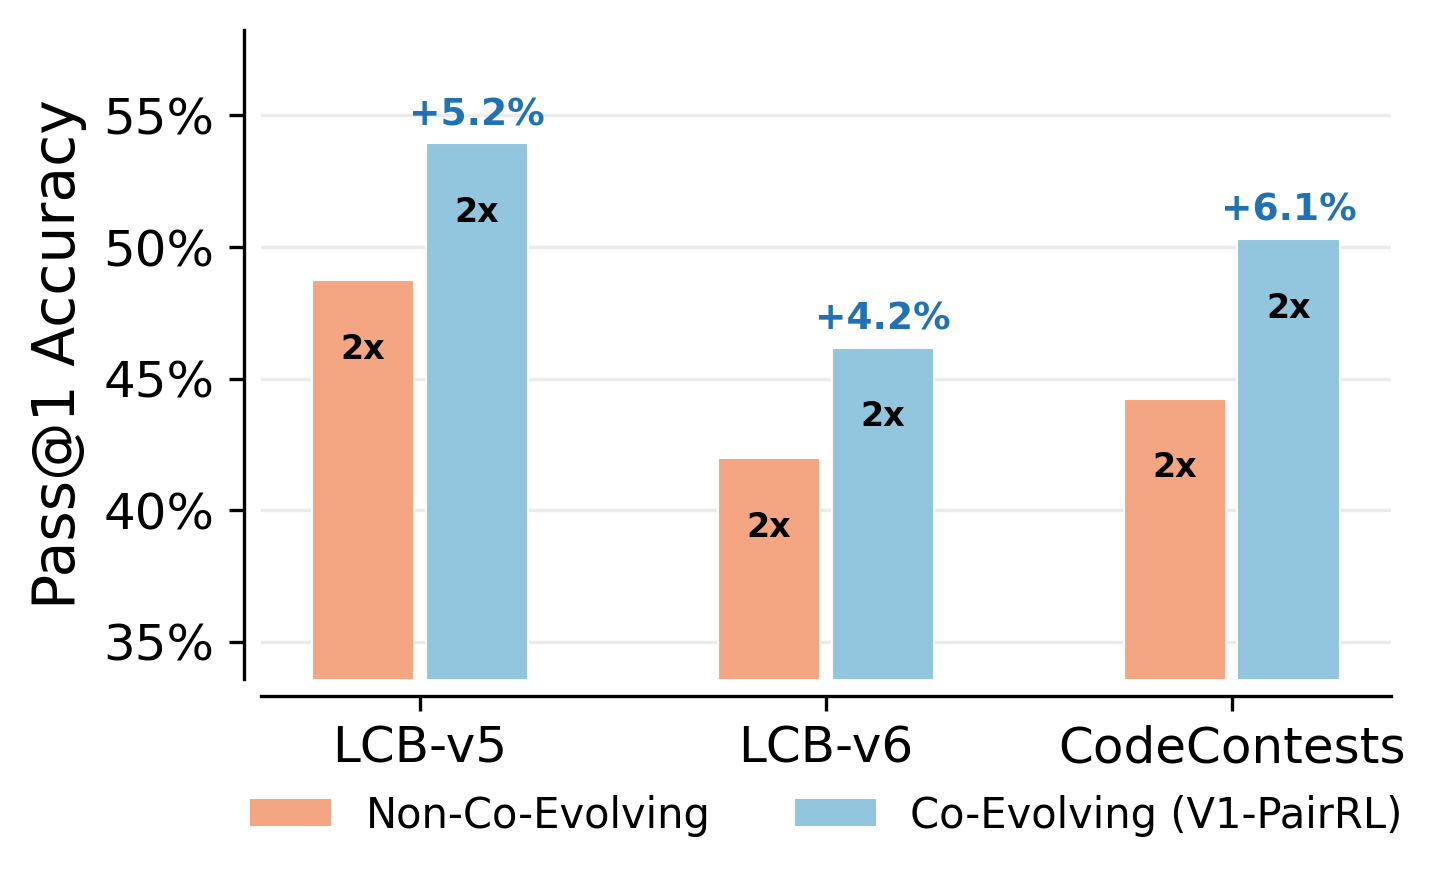
\includegraphics[width=0.43\textwidth]{images_verif/coevolving_vs_noncoevolving_ablation.png}
    \caption{Co-evolving vs.\ non-co-evolving pairwise verification. Both use \pairinfer{} (2x budget).}
    \label{fig:coevolving_ablation}
    % \vspace{-2em}
\end{wrapfigure}
\textbf{Co-evolving training is critical for inducing strong pairwise self-verification capabilities.}
\method{}-PairRL trains solution generation and verification capabilities in a co-evolving setup where the model is trained for self-verification using samples generated online at the same iteration thus adapting to its own evolving generation distribution. An alternative way of jointly optimizing these capabilities is to train the model in a multi-task setup where the data for the verification task is generated offline, using the base model, before training.
To isolate the effect of co-evolving training, we train a \textit{non-co-evolving} baseline: the same model trained with RL for generation as well as verification. For this, we first run the Qwen3-4B-Instruct-2507 model on the DeepCoder dataset prompts to generate 8 solutions per prompt, and then use these solutions as part of the verifier prompt during RL training. We apply \pairinfer{} at inference time with the same 2x budget. As shown in Figure~\ref{fig:coevolving_ablation}, co-evolving training consistently outperforms the non-co-evolving setup across all benchmarks.

\par\vspace{\intextsep}
\noindent\begin{minipage}{\textwidth}
\begin{tcolorbox}[title=Takeaway: Co-Training Generation and Pairwise Self-Verification, colback=green!5]
Unified RL training that jointly optimizes generation and pairwise verification (\method{}-PairRL) produces stronger reasoning models and improves test-time scaling compared with generation-only baselines or models co-trained with pointwise verification.
\end{tcolorbox}
\end{minipage}


